% ===================================================================================== %
%                                        Header                                         %
% ===================================================================================== %
\documentclass[10pt,t,xcolor=table]{beamer}

\usepackage[T1]{fontenc}
\usepackage{textcomp}
\usepackage{lmodern}
\usepackage{amsmath}
\usepackage{setspace}
\usepackage{ifthen}
\usepackage{xspace}
\usepackage{booktabs}
\usepackage{multirow}
\usepackage{appendixnumberbeamer}


\makeatletter
\beamer@compresstrue
\makeatother
\useoutertheme{miniframes}
\usecolortheme{beaver}
\useinnertheme{circles}
\setbeamertemplate{navigation symbols}{}%remove navigation symbols

\setbeamercolor{itemize item}{fg=darkred}
\setbeamercolor{itemize subitem}{fg=darkred}
\setbeamercolor{section number projected}{bg=darkred}

\setbeamertemplate{footline}{%
    \begin{beamercolorbox}[leftskip=0.5em,rightskip=0.5em]{palette primary}
        \vskip0.3em
        \ifx \TheDepartmentShort \Undefined
            \TheAuthorShort\hfill \TheInstituteShort
        \else
            \TheAuthorShort\hfill \TheDepartmentShort | \TheInstituteShort
        \fi
        \vskip0.3em
    \end{beamercolorbox}
    
    \begin{beamercolorbox}[leftskip=0.5em,rightskip=0.5em]{section in head/foot}
        \vskip0.3em
        \TheTitleShort \hfill \insertframenumber/\inserttotalframenumber
        \vskip0.3em
    \end{beamercolorbox}%
}





% =============================================================================================== %
%                                     Math Commands                                               %
% =============================================================================================== %


% ---------------------------------------------------------------------------- %
%                                Square Root Tail                              %
% ---------------------------------------------------------------------------- %
\DeclareRobustCommand{\NthRootInTeX}[2]{\root #1 \of {#2\:\!}}

\DeclareRobustCommand{\SquareRootCore}[2]{
    \setbox0=\hbox{\ensuremath{\NthRootInTeX{#1}{#2}}}
    \dimen0=\ht0
    \advance\dimen0-0.2\ht0
    \setbox2=\hbox{\vrule height\ht0 depth -\dimen0}
    {\box0\lower0.47pt\box2}
}

\DeclareRobustCommand{\Sqrt}[2][]{
    \mathchoice{\SquareRootCore{#1}{#2}}
               {\SquareRootCore{#1}{#2}}
               {\SquareRootCore{#1}{#2}}
               {\SquareRootCore{#1}{#2}}
}



% ---------------------------------------------------------------------------- %
%                              Derivative Commands                             %
% ---------------------------------------------------------------------------- %
\newcommand{\bigdiffn}[4]{\dfrac{#1{}^{#4}}{#1 #3{}^{#4}} \left[ #2 \right]}
\newcommand{\gendiffn}[4]{\dfrac{#1{}^{#4} #2}{#1 #3{}^{#4}}}

\newcommand{\diff}[3][d]{
    \ifthenelse{\equal{p}{#1}}{
        \gendiffn{\partial}{#2}{#3}{}
    }{
        \ifthenelse{\equal{b}{#1}}{
            \bigdiffn{d}{#2}{#3}{}
        }{
            \ifthenelse{\equal{bp}{#1}}{
                \bigdiffn{\partial}{#2}{#3}{}
            }{
                \gendiffn{d}{#2}{#3}{}
            }
        }
    }
}

\newcommand{\diffn}[4][d]{
    \ifthenelse{\equal{p}{#1}}{
        \gendiffn{\partial}{#2}{#3}{#4}
    }{
        \ifthenelse{\equal{b}{#1}}{
            \bigdiffn{#2}{#3}{#4}
        }{
            \ifthenelse{\equal{bp}{#1}}{
                \bigdiffn{\partial}{#2}{#3}{#4}
            }{
                \gendiffn{#1}{#2}{#3}{#4}
            }
        }
    }
}

\newcommand{\bigdiff}   [2] {\diff[b]{#1}{#2}}
\newcommand{\pdiff}     [2] {\diff[p]{#1}{#2}}
\newcommand{\bigpdiff}  [2] {\diff[bp]{#1}{#2}}
\let\frac\dfrac
\newcommand{\subs}      [2][]{\ensuremath{{}_{#1\text{\scriptsize #2}}}}
\newcommand{\sups}      [2][]{\ensuremath{{}^{#1\text{\scriptsize #2}}}}
\newcommand{\oneo}      [1]  {\ensuremath{\frac{1}{#1}}}




\newcommand{\Density}{\ensuremath{\rho}\xspace}
\newcommand{\Temperature}{\ensuremath{T}\xspace}
\newcommand{\Pressure}{\ensuremath{P}\xspace}
\newcommand{\IntEnergy}{\ensuremath{i}\xspace}
\newcommand{\Entropy}{\ensuremath{s}\xspace}
\newcommand{\Enthalpy}{\ensuremath{h}\xspace}
\newcommand{\ThCond}{\kappa}
\newcommand{\Viscosity}{\mu}
\newcommand{\DiffCoef}{\ensuremath{D}\xspace}

\newcommand{\isat}{\ensuremath{\IntEnergy\subs[\!]{sat}}\xspace}
\newcommand{\Psat}{\ensuremath{\Pressure\subs[\!\!]{sat}}\xspace}
\newcommand{\Tsat}{\ensuremath{\Temperature\subs[\!\!\:]{sat}}\xspace}
\newcommand{\SubL}{\subs[\!\!\:]{\rule{0pt}{8pt}$\textstyle\ell$}}
\newcommand{\SubG}{\subs[\!\!\:]{$\mathit{g}$}}

\newcommand{\rhol}{\ensuremath{\rho\SubL}\xspace}
\newcommand{\rhog}{\ensuremath{\rho\SubG}\xspace}
\newcommand{\il}{\ensuremath{i\SubL}\xspace}
\newcommand{\ig}{\ensuremath{i\SubG}\xspace}
\newcommand{\rhoul}{\ensuremath{\rhou\SubL}\xspace}
\newcommand{\rhoug}{\ensuremath{\rhou\SubG}\xspace}
\newcommand{\rhoil}{\ensuremath{\rhoi\SubL}\xspace}
\newcommand{\rhoig}{\ensuremath{\rhoi\SubG}\xspace}
\newcommand{\alphal}{\ensuremath{\alpha\SubL}\xspace}
\newcommand{\alphag}{\ensuremath{\alpha\SubG}\xspace}

\newcommand{\tauSat}{\ensuremath{\tau\subs[\!\!\:]{sat}}\xspace}
\newcommand{\deltaL}{\ensuremath{\delta\subs[\!\!\:]{\rule{0pt}{8pt}$\textstyle\ell$}}\xspace}
\newcommand{\deltaG}{\ensuremath{\delta\subs[\!\!\:]{$\mathit{g}$}}\xspace}

\newcommand{\rhoc}  {\ensuremath{\rho\subs{c}}\xspace}
\newcommand{\Tc}    {\ensuremath{T\subs{c}}\xspace}

\newcommand{\Skip}[1][0.45em]{\\[#1]}
\newcommand{\TCS}    {Thermodynamic Coexistence System\xspace}
\newcommand{\TCSRef} {\hyperref[Eqn:TCS]{\TCS}\xspace}
\newcommand{\MCS}    {Mechanical Coexistence System\xspace}
\newcommand{\MCSRef} {\hyperref[Eqn:MCS]{\MCS}\xspace}

\newcommand{\Afe}{\ensuremath{A\subs{\textsc{fe}}}}
\newcommand{\HFE}{Helmholtz free energy\xspace}
\newcommand{\EOS}{equation of state\xspace}

\newcommand{\Space}{\ensuremath{z}\xspace}
\newcommand{\Time}{\ensuremath{t}\xspace}
\newcommand{\Speeds}{\ensuremath{\mathbf{\lambda}}\xspace}

\DeclareMathOperator{\Ln}{Ln}
\DeclareMathOperator{\Abs}{Abs}
\DeclareMathOperator{\Inf}{Inf}
\DeclareMathOperator{\Exp}{Exp}
\DeclareMathOperator{\Rez}{R}

\let\originalleft\left
\let\originalright\right
\renewcommand{\left}{\mathopen{}\mathclose\bgroup\originalleft\;\!}
\def\left#1{\mathopen{}\mathclose\bgroup\originalleft#1\:\!}
\def\right#1{\aftergroup\egroup\:\!\originalright#1}


%\DefineNewLength{\RowSkip}{1.0em}
%\newcommand{\skp}[1][0.45em]{
%    \ifthenelse{\equal{#1}{}}{
%        \\[\RowSkip]
%    }{
%        \\[#1]
%    }
%}

\newcommand{\Del}[1][]{
    \partial_{#1}
}

\newcommand{\Vector}[1]{
    \underline{#1}
}

\newcommand{\Tensor}[1]{
    \underline{\underline{#1}}
}

\newcommand{\qConRaw}{\mathbf{q}}
\newcommand{\qCon}{\ensuremath{\qConRaw}\xspace}
\newcommand{\qPer}{\ensuremath{\widehat{\qConRaw}}\xspace}
\newcommand{\qSS} {\ensuremath{\qConRaw^0}\xspace}

\newcommand{\ConSys}{
    \Psi
}

\newcommand{\ConSysHEM}[1][HEM]{
    \ConSys_{\!\mbox{\tiny #1}}
}


\newcommand{\Flux}{
    \mathbf{F}
}
\newcommand{\Source}{
    \mathbf{S}
}

\newcommand{\Weight}{\beta}


\newcommand{\FluxFun}[2][]{
    \mathbf{F}_{#1}\left(#2\right)
}

\newcommand{\SourceFun}[2][]{
    \mathbf{S}_{#1}\left(#2\right)
}

\newcommand{\ResidualFun}[2][]{
    \mathbf{R}_{#1}\left(#2\right)
}

\newcommand{\Jacobian}[1][]{
    \mathbb{J}\subs{#1}
}

\newcommand{\JacobGen}[2]{
  \Jacobian[{\scriptscriptstyle #1}](#2)
}

\newcommand{\JacobF}{
    \Jacobian[F]
}


\newcommand{\JacobS}[1]{
    \JacobGen{S}{#1}
}

\newcommand{\FluxSS}{
    \mathbf{F}^{0}
}

\newcommand{\SourceSS}{
    \mathbf{S}^{0}
}

\newcommand{\JacobFSS}[1][\,\,\!]{
    \mathbf{J}_{\!{\scriptscriptstyle F}}^{0}{}#1
}

\newcommand{\JacobSSS}[1][\,\,\!]{
    \mathbf{J}_{\!{\scriptscriptstyle S}}^{0}#1
}

\newcommand{\BigO}[1]{
    \ensuremath{\mathcal{O}\!\left(#1\right)}
}


\newcommand{\Correl}[2]{
    f^{\mbox{\scriptsize cor}}_{#1}\left(#2\right)
}

\newcommand{\LpNorm}[2][2]{
    \ensuremath{\lvert\!\lvert#2\rvert\!\rvert_{#1}}
}

\newcommand{\Nudge}{
    \ensuremath{\!\!\;}
}

\newcommand{\hfg}{
    \ensuremath{h_{\mbox{\scriptsize fg}}}
}



%\NewEnviron{BoxedAlgorithm}[1][H]{
%    \begin{center}
%        \begin{minipage}{0.999\textwidth}
%            \centering
%            \fcolorbox{black}{white}{
%                \centering
%                \begin{minipage}[t]{0.85\textwidth}
%                    \begin{algorithm}[#1]
%                        \BODY
%                    \end{algorithm}
%                \end{minipage}
%            }
%        \end{minipage}
%    \end{center}
%}


\DeclareRobustCommand{\TH}  {thermal hydraulics\xspace}
\DeclareRobustCommand{\THc} {Thermal hydraulics\xspace}
\DeclareRobustCommand{\THcc}{Thermal Hydraulics\xspace}
\DeclareRobustCommand{\THs} {thermal hydraulic\xspace}

\DeclareRobustCommand{\CLaw}  {conservation law\xspace}
\DeclareRobustCommand{\CLaws} {conservation laws\xspace}


\newcommand{\rhou}{\ensuremath{\rho{u}}\xspace}
\newcommand{\rhoi}{\ensuremath{\rho{i}}\xspace}

\newcommand{\tr}{\ensuremath{{}\sups{\textsc{T}}}}
\newcommand{\mdotloss}[1][]{\ensuremath{\dot{m}'''\subs[\!\!\!\!\!#1]{loss}}\xspace}
\newcommand{\Keff}{\ensuremath{K\subs{eff}}}

\newcommand{\POfRhoRhoi}{\ensuremath{P\left(\rho,\frac{\rhoi}{\rho}\right)}}


\newcommand{\EqnSkip}[1][3em]{\ensuremath{\mbox{\rule{0.5em}{#1}}}\\}
\newcommand{\psiEOS}{\ensuremath{\psi}\subs{\textsc{eos}}}




%\DefineNewLength{\BarredLetterHeight}{0pt}
%\DefineNewLength{\BarredLetterWidth}{0pt}

%\newcommand{\eBB}{
%    \ensuremath{
%        \settoheight{\BarredLetterHeight}{e} % Height in current context
%        \settowidth{\BarredLetterWidth}{e}   % Width  in current context
%        e\mbox{\hspace{-0.57\BarredLetterWidth}\rule{0.035em}{0.96\BarredLetterHeight}} % bar
%    }
%}

%\newcommand{\TableSkip}{\rule[-1.4em]{0pt}{3.3em} \\[0pt]}
\definecolor{Gray}{gray}{0.93}


\newcommand{\LedineggCriterion}{$\tfrac{\partial\Delta{P}}{\partial(\rhou)}\bigr\rvert_{\text{int}} \le 
                                 \tfrac{\partial\Delta{P}}{\partial(\rhou)}\bigr\rvert_{\text{ext}}$}
                                
                                
\newcommand{\etal}{et al.\xspace}
\newcommand{\etc}{etc.\xspace}
\newcommand{\eg}{e.g.\xspace}
\newcommand{\ie}{i.e.\xspace}


\newcommand{\rhok}{ \ensuremath{\alpha\rho\subs{\phi}}\xspace}
\newcommand{\rhouk} {\ensuremath{\alpha\rhou\subs{\phi}}\xspace}
\newcommand{\rhoik} {\ensuremath{\alpha\rhoi\subs{\phi}}\xspace}
\newcommand{\alphak}{\ensuremath{\alpha\subs{\phi}\xspace}}
\newcommand{\uk}{\ensuremath{u\subs{\phi}}\xspace}
\newcommand{\ik}{\ensuremath{i\subs{\phi}}\xspace}
\newcommand{\CVvol}[1][k]{\ensuremath{\Omega_\text{#1}}\xspace}
\newcommand{\MCvol}[1][m]{\ensuremath{\Omega_\text{#1}}\xspace}
\newcommand{\CVsurf}[1][k]{\ensuremath{\Gamma_\text{#1}}\xspace}
\newcommand{\MCsurf}[1][m]{\ensuremath{\Gamma_\text{#1}}\xspace}








    \let\Oldalpha     \alpha     \renewcommand{\alpha}     {\ensuremath{\Oldalpha     }\xspace}
    \let\Oldbeta      \beta      \renewcommand{\beta}      {\ensuremath{\Oldbeta      }\xspace}
    \let\Oldgamma     \gamma     \renewcommand{\gamma}     {\ensuremath{\Oldgamma     }\xspace}
    \let\Olddelta     \delta     \renewcommand{\delta}     {\ensuremath{\Olddelta     }\xspace}
    \let\Oldepsilon   \epsilon   \renewcommand{\epsilon}   {\ensuremath{\Oldepsilon   }\xspace}
    \let\Oldvarepsilon\varepsilon\renewcommand{\varepsilon}{\ensuremath{\Oldvarepsilon}\xspace}
    \let\Oldzeta      \zeta      \renewcommand{\zeta}      {\ensuremath{\Oldzeta      }\xspace}
    \let\Oldeta       \eta       \renewcommand{\eta}       {\ensuremath{\Oldeta       }\xspace}
    \let\Oldtheta     \theta     \renewcommand{\theta}     {\ensuremath{\Oldtheta     }\xspace}
    \let\Oldvartheta  \vartheta  \renewcommand{\vartheta}  {\ensuremath{\Oldvartheta  }\xspace}
    \let\Oldkappa     \kappa     \renewcommand{\kappa}     {\ensuremath{\Oldkappa     }\xspace}
    \let\Oldlambda    \lambda    \renewcommand{\lambda}    {\ensuremath{\Oldlambda    }\xspace}
    \let\Oldmu        \mu        \renewcommand{\mu}        {\ensuremath{\Oldmu        }\xspace}
    \let\Oldnu        \nu        \renewcommand{\nu}        {\ensuremath{\Oldnu        }\xspace}
    \let\Oldxi        \xi        \renewcommand{\xi}        {\ensuremath{\Oldxi        }\xspace}
    \let\Oldpi        \pi        \renewcommand{\pi}        {\ensuremath{\Oldpi        }\xspace}
    \let\Oldvarpi     \varpi     \renewcommand{\varpi}     {\ensuremath{\Oldvarpi     }\xspace}
    \let\Oldrho       \rho       \renewcommand{\rho}       {\ensuremath{\Oldrho       }\xspace}
    \let\Oldvarrho    \varrho    \renewcommand{\varrho}    {\ensuremath{\Oldvarrho    }\xspace}
    \let\Oldsigma     \sigma     \renewcommand{\sigma}     {\ensuremath{\Oldsigma     }\xspace}
    \let\Oldvarsigma  \varsigma  \renewcommand{\varsigma}  {\ensuremath{\Oldvarsigma  }\xspace}
    \let\Oldtau       \tau       \renewcommand{\tau}       {\ensuremath{\Oldtau       }\xspace}
    \let\Oldupsilon   \upsilon   \renewcommand{\upsilon}   {\ensuremath{\Oldupsilon   }\xspace}
    \let\Oldphi       \phi       \renewcommand{\phi}       {\ensuremath{\Oldphi       }\xspace}
    \let\Oldvarphi    \varphi    \renewcommand{\varphi}    {\ensuremath{\Oldvarphi    }\xspace}
    \let\Oldchi       \chi       \renewcommand{\chi}       {\ensuremath{\Oldchi       }\xspace}
    \let\Oldpsi       \psi       \renewcommand{\psi}       {\ensuremath{\Oldpsi}\xspace}
    \let\Oldomega     \omega     \renewcommand{\omega}     {\ensuremath{\Oldomega     }\xspace}
    \let\OldGamma     \Gamma     \renewcommand{\Gamma}     {\ensuremath{\OldGamma     }\xspace}
    \let\OldLambda    \Lambda    \renewcommand{\Lambda}    {\ensuremath{\OldLambda    }\xspace}
    \let\OldSigma     \Sigma     \renewcommand{\Sigma}     {\ensuremath{\OldSigma     }\xspace}
    \let\OldPsi       \Psi       \renewcommand{\Psi}       {\ensuremath{\OldPsi       }\xspace}
    \let\OldDelta     \Delta     \renewcommand{\Delta}     {\ensuremath{\OldDelta     }\xspace}
    \let\OldXi        \Xi        \renewcommand{\Xi}        {\ensuremath{\OldXi        }\xspace}
    \let\OldUpsilon   \Upsilon   \renewcommand{\Upsilon}   {\ensuremath{\OldUpsilon   }\xspace}
    \let\OldOmega     \Omega     \renewcommand{\Omega}     {\ensuremath{\OldOmega     }\xspace}
    \let\OldTheta     \Theta     \renewcommand{\Theta}     {\ensuremath{\OldTheta     }\xspace}
    \let\OldPi        \Pi        \renewcommand{\Pi}        {\ensuremath{\OldPi        }\xspace}
    \let\OldPhi       \Phi       \renewcommand{\Phi}       {\ensuremath{\OldPhi       }\xspace}


\setlength{\parskip}{0.5em}

\def\Empty{}
\newlength{\LengthOfArgument}
\newcommand{\IfEmpty}[3]{
    \settowidth{\LengthOfArgument}{#1}
    \ifdim\LengthOfArgument=0pt
        #2
    \else
        #3
    \fi
}

\newcommand{\Author}[2][]{

    \IfEmpty{#1}{
        \def\TheAuthorShort{#2\xspace}
        \def\TheAuthorLong{#2\xspace}
        \author{#2}
    }{
        \def\TheAuthorShort{#1\xspace}
        \def\TheAuthorLong{#2\xspace}
        \author[#1]{#2}
    }
}

\newcommand{\Institute}[2][]{

    \IfEmpty{#1}{
        \def\TheInstituteShort{#2\xspace}
        \def\TheInstituteLong{#2\xspace}
        \institute{#2}
    }{
        \def\TheInstituteShort{#1\xspace}
        \def\TheInstituteLong{#2\xspace}
        \institute[#1]{#2}
    }
}

\newcommand{\Title}[2][]{

    \IfEmpty{#1}{
        \def\TheTitleShort{#2\xspace}
        \def\TheTitleLong{#2\xspace}
        \title{#2}
    }{
        \def\TheTitleShort{#1\xspace}
        \def\TheTitleLong{#2\xspace}
        \title[#1]{#2}
    }
}

\newcommand{\Department}[2][]{

    \IfEmpty{#1}{
        \def\TheDepartmentShort{#2\xspace}
        \def\TheDepartmentLong{#2\xspace}
    }{
        \def\TheDepartmentShort{#1\xspace}
        \def\TheDepartmentLong{#2\xspace}
    }
}






\newenvironment{Itemize}
    {\begin{itemize}\setlength{\itemsep}{0.8em}\setlength{\leftmargin}{0.0em}\setlength{\labelwidth}{0em}}
    {\end{itemize}}



%\title{On the Stability of Natural Circulation Loops with Phase Change}
\Title{On the Behavior of Natural Circulation Loops with Phase Change}
\Institute{University of Wisconsin--Madison}
\Department{Engineering Physics Department}
\Author{Troy C. Haskin}
\date{12/17/2012}

\graphicspath{{./Graphics/}}

\AtBeginSection[]{
    \begin{frame}<beamer>
        \tableofcontents[currentsection]
    \end{frame}
}
\AtBeginSubsection[]{
    \ifnum\value{subsection} > 1
        \begin{frame}<beamer>
            \tableofcontents[currentsection,currentsubsection]
        \end{frame}
    \fi
}


\logo{\vspace{0.5em}
\includegraphics[scale=0.2]{Picture1}}


% =========================================================================== %
%                              Document                                       %
% =========================================================================== %
\begin{document}


% ======================================================= %
%                         Titlepage                       %
% ======================================================= %
\begin{frame}
    \titlepage
\end{frame}


% ======================================================= %
%                         Outline                         %
% ======================================================= %
\section*{Outline}
\begin{frame}
    \tableofcontents
\end{frame}



% ======================================================= %
%                       Introduction                      %
% ======================================================= %
\chapter{Introduction}

Stability of two-phase natural circulation systems is not a novel subject in-and-of itself.
However, this work aims to perform the analysis on a closed-loop geometry with unique characteristics to be discussed.
Motivation for this effort will be given from examination of a physical system.
Then, a literature review will be given that overviews the field of stability analysis in general.
Finally, some concluding remarks will be given pertaining to the goals of this work.

\IncludeSection{Section2-ReactorCavityCoolingSystem}
\newpage
\IncludeSection{Section3-Literature}

\section{Research Purpose}\label{Section:Purpose}

The contribution of this work to the two-phase stability literature is a combination of topics in one analysis.
First, this work uses a non-ideal, continuous \Acro{EOS} for water.
Rather than approximating liquid water as a stiffened gas \cite{hayward_compressibility_1967-1} or using tabulated values, a complete implementation of the equation of state of water from the \Acro{IAPWS} is used.
All thermodynamic and kinematic properties used in the simulations are calculated from the mechanically balanced mass and energy of the system.
Second, this work uses an implementation of a modern, nonlinear solver that accurately and conservatively calculates all of the steady-states from which the linear stability calculations are made.
The solver is based on Newton-Raphson methods but avoids the need to form the true Jacobian of the system during simulation, which greatly decreases the computational cost of the solution.
Third, a modified discretization scheme is presented.
It is a scheme that aims to allow complete physical coverage of the computational domain by a course, staggered grid and therefore allow complete and correct integration of the physical domain on both the conservation and momentum fields.
This proper integration allows for a mathematically rigorous integration of the domain for accurate calculation of linear stability via full domain integration.
The final result of these efforts is a stability analysis of a simple, closed-loop system under different power loads in both single and two-phase states.










% ======================================================= %
%                     Preliminary Work                    %
% ======================================================= %
\section{Preliminary Work}
    
    \subsection{MELCOR Simulations}
    % --------------------------------------------------- %
    %               RCCS: MELCOR  Simulations             %
    % --------------------------------------------------- %
    \begin{frame}[label=MassFlowAnnotate]{Full-scale model under accident conditions}
        \hspace{4.9em}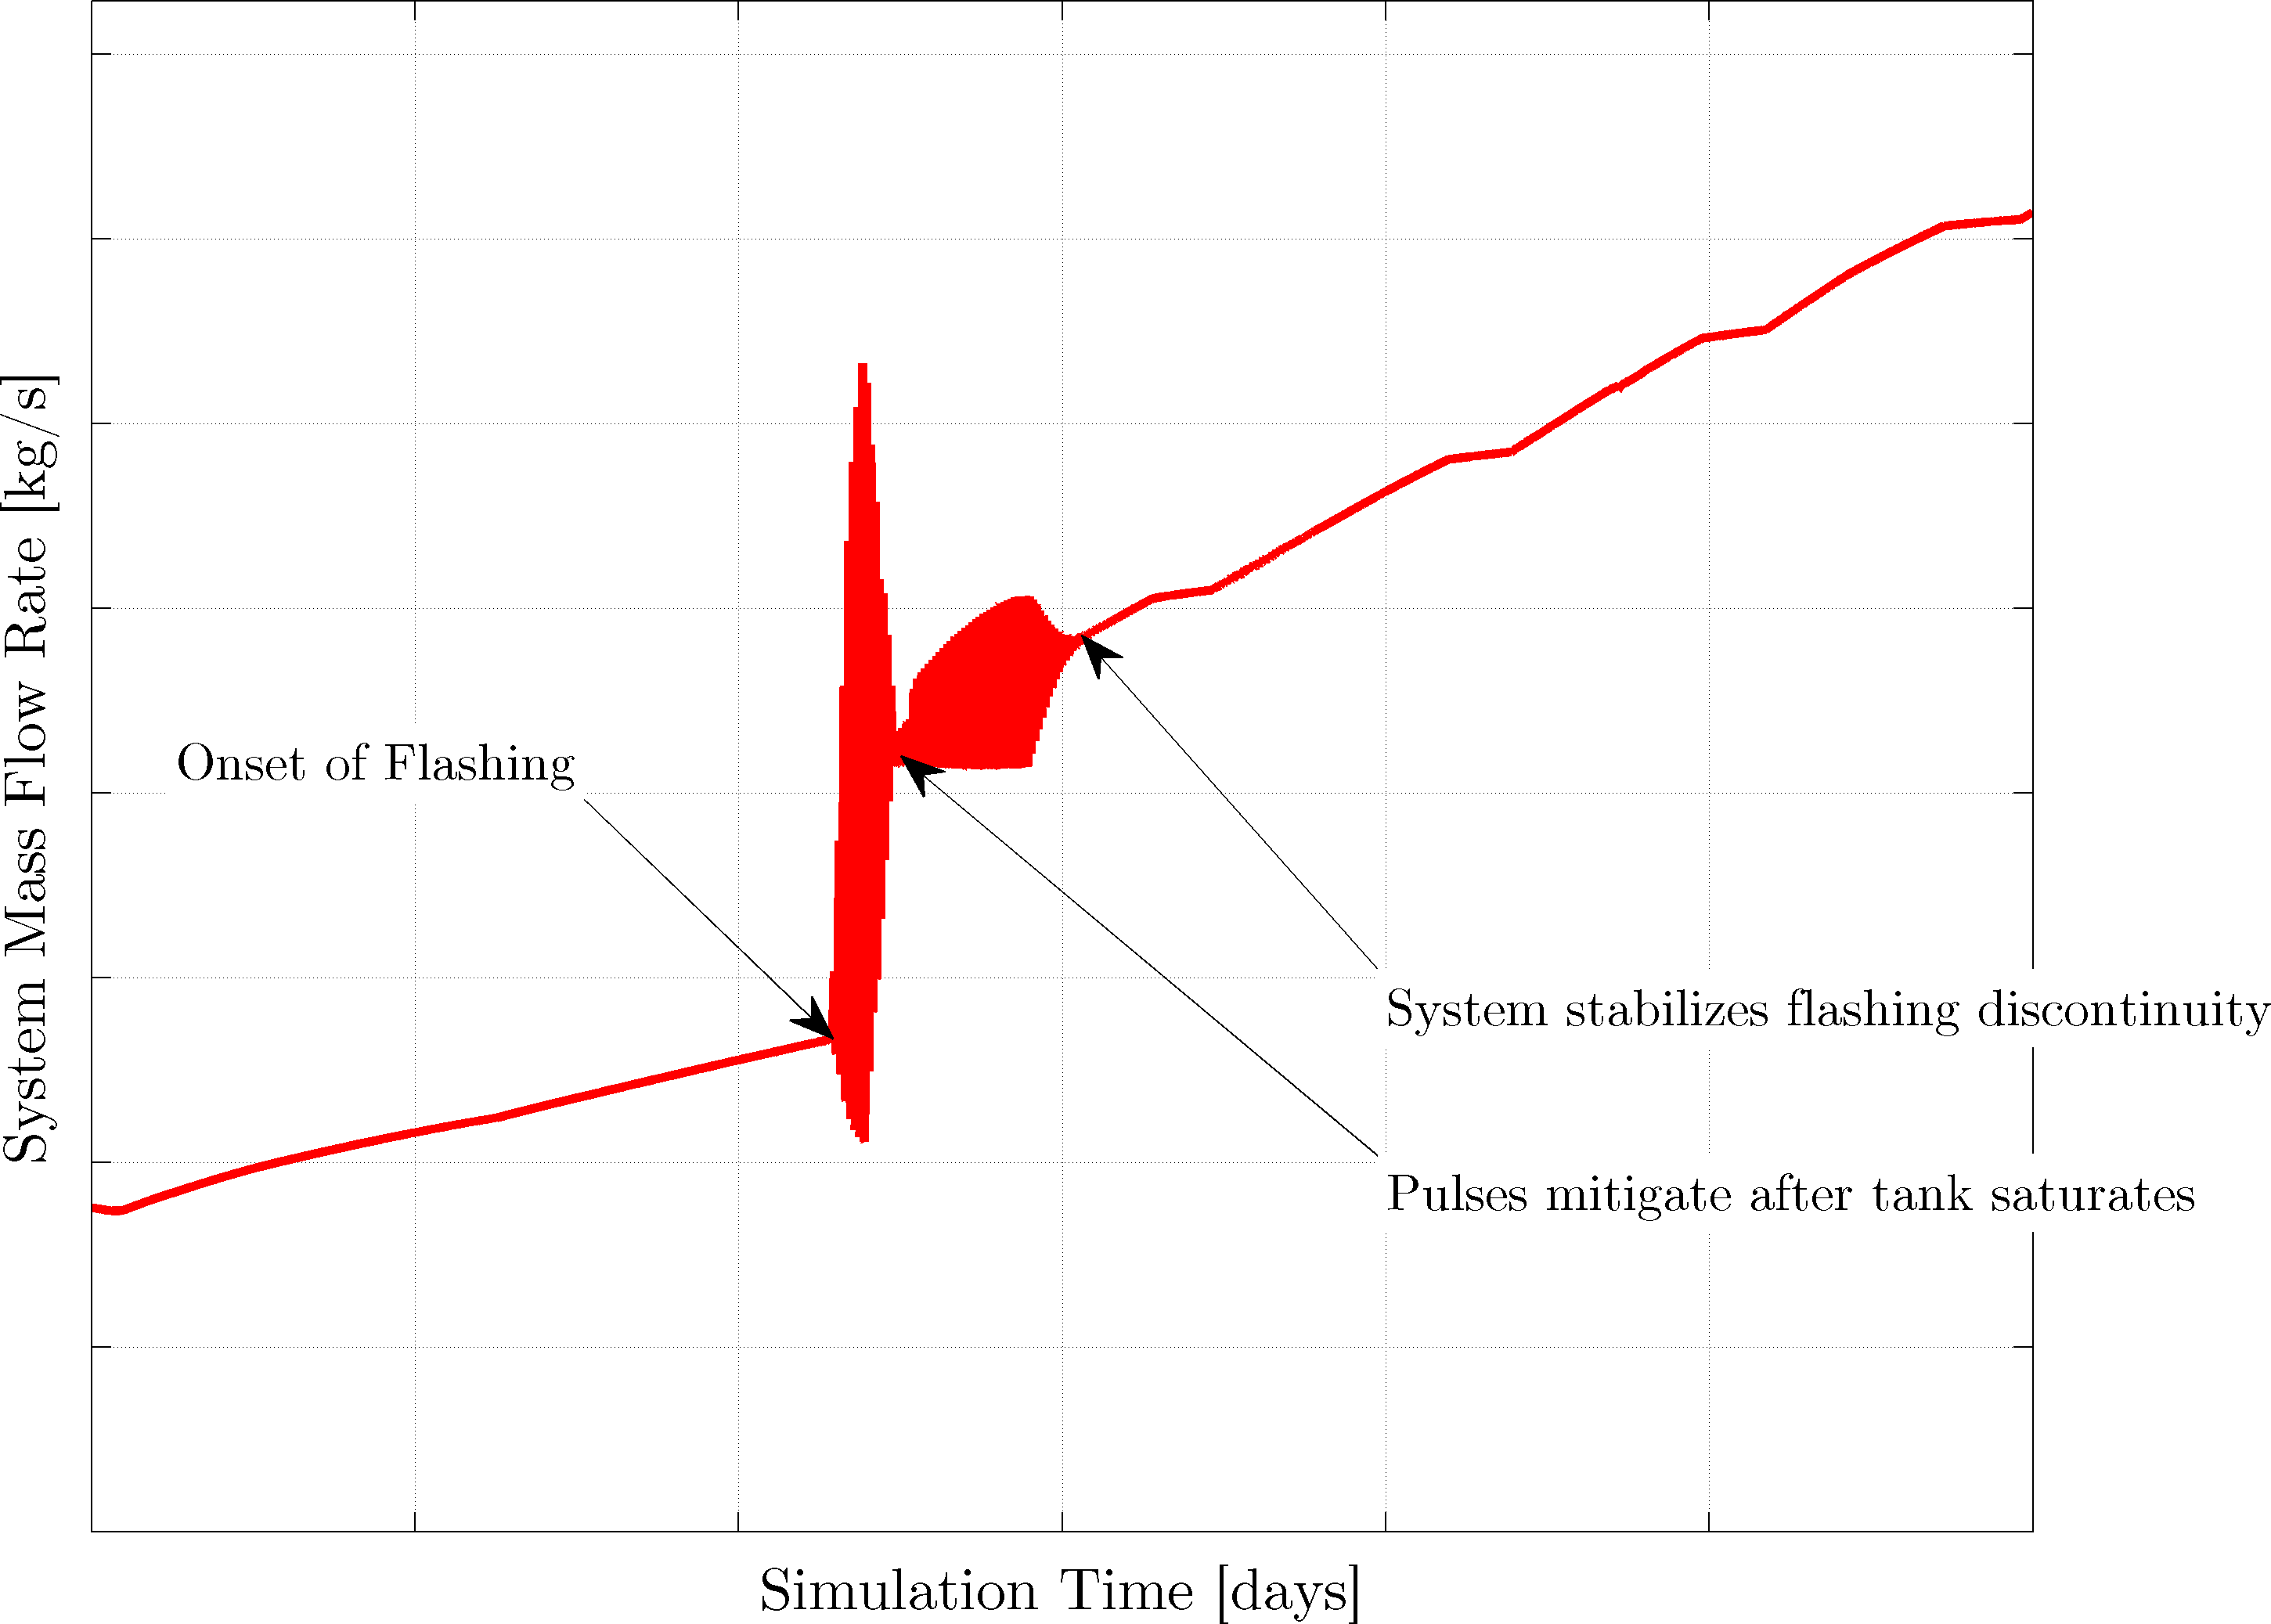
\includegraphics[height=2.4in]{PowerProfiles_MassFlowRateAnnotationsThesis}
        
        \hfill\textit{\tiny\hyperlink{MassFlow4Days}{alternate}}
    \end{frame}



    % --------------------------------------------------- %
    %             RCCS:Mass Flow rate Simulation          %
    % --------------------------------------------------- %
    \begin{frame}[c]{RCCS Experiment: Model Simulation}
        \begin{columns}[c]
            \begin{column}{0.28\textwidth}
                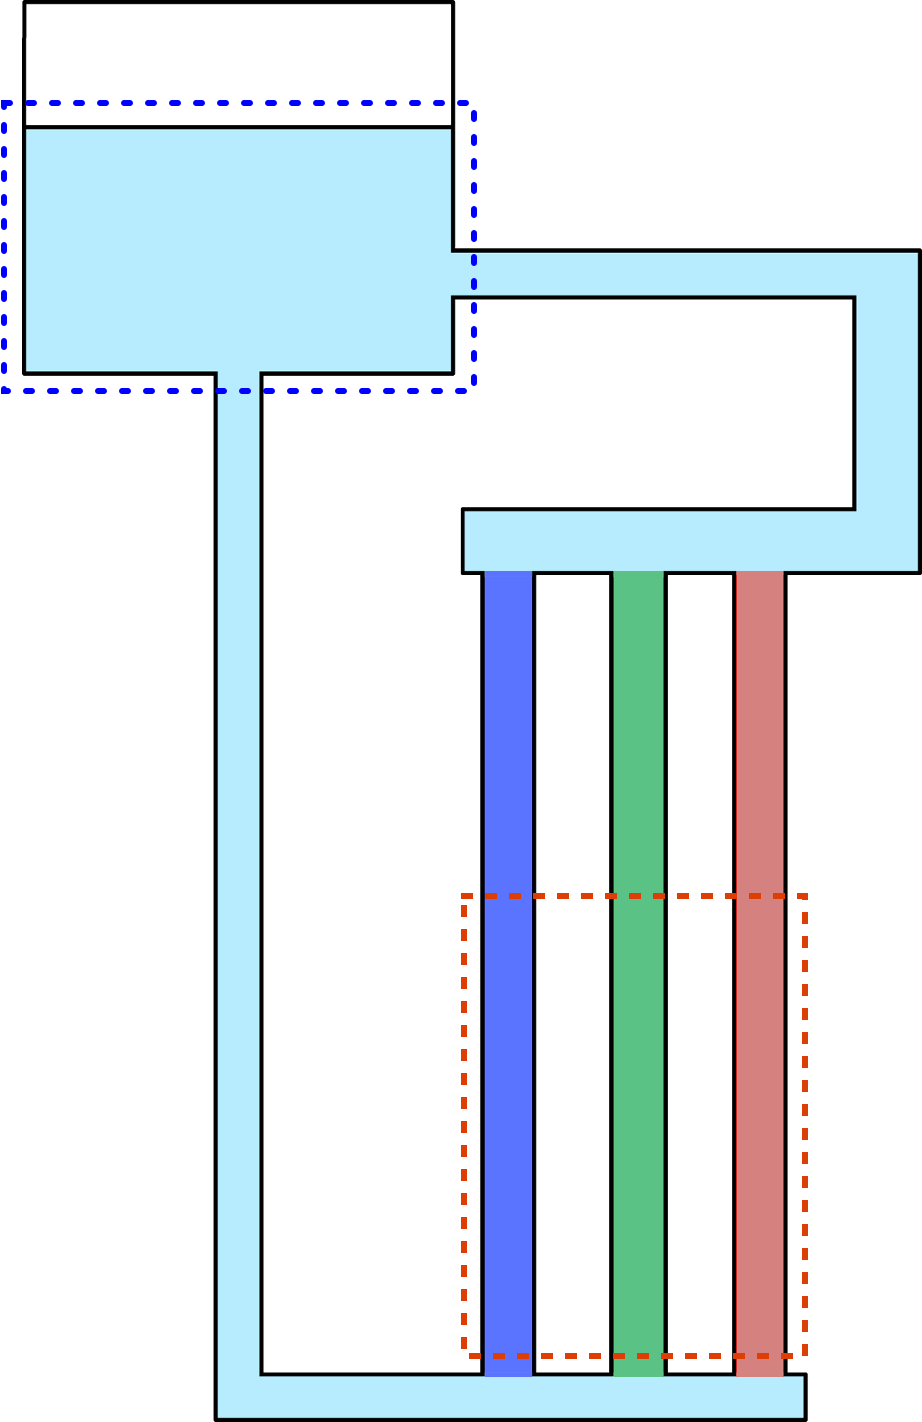
\includegraphics[height=1.8in]{RCCSExperimentRiserPlotAid}
            \end{column}
            \begin{column}{0.65\textwidth}
                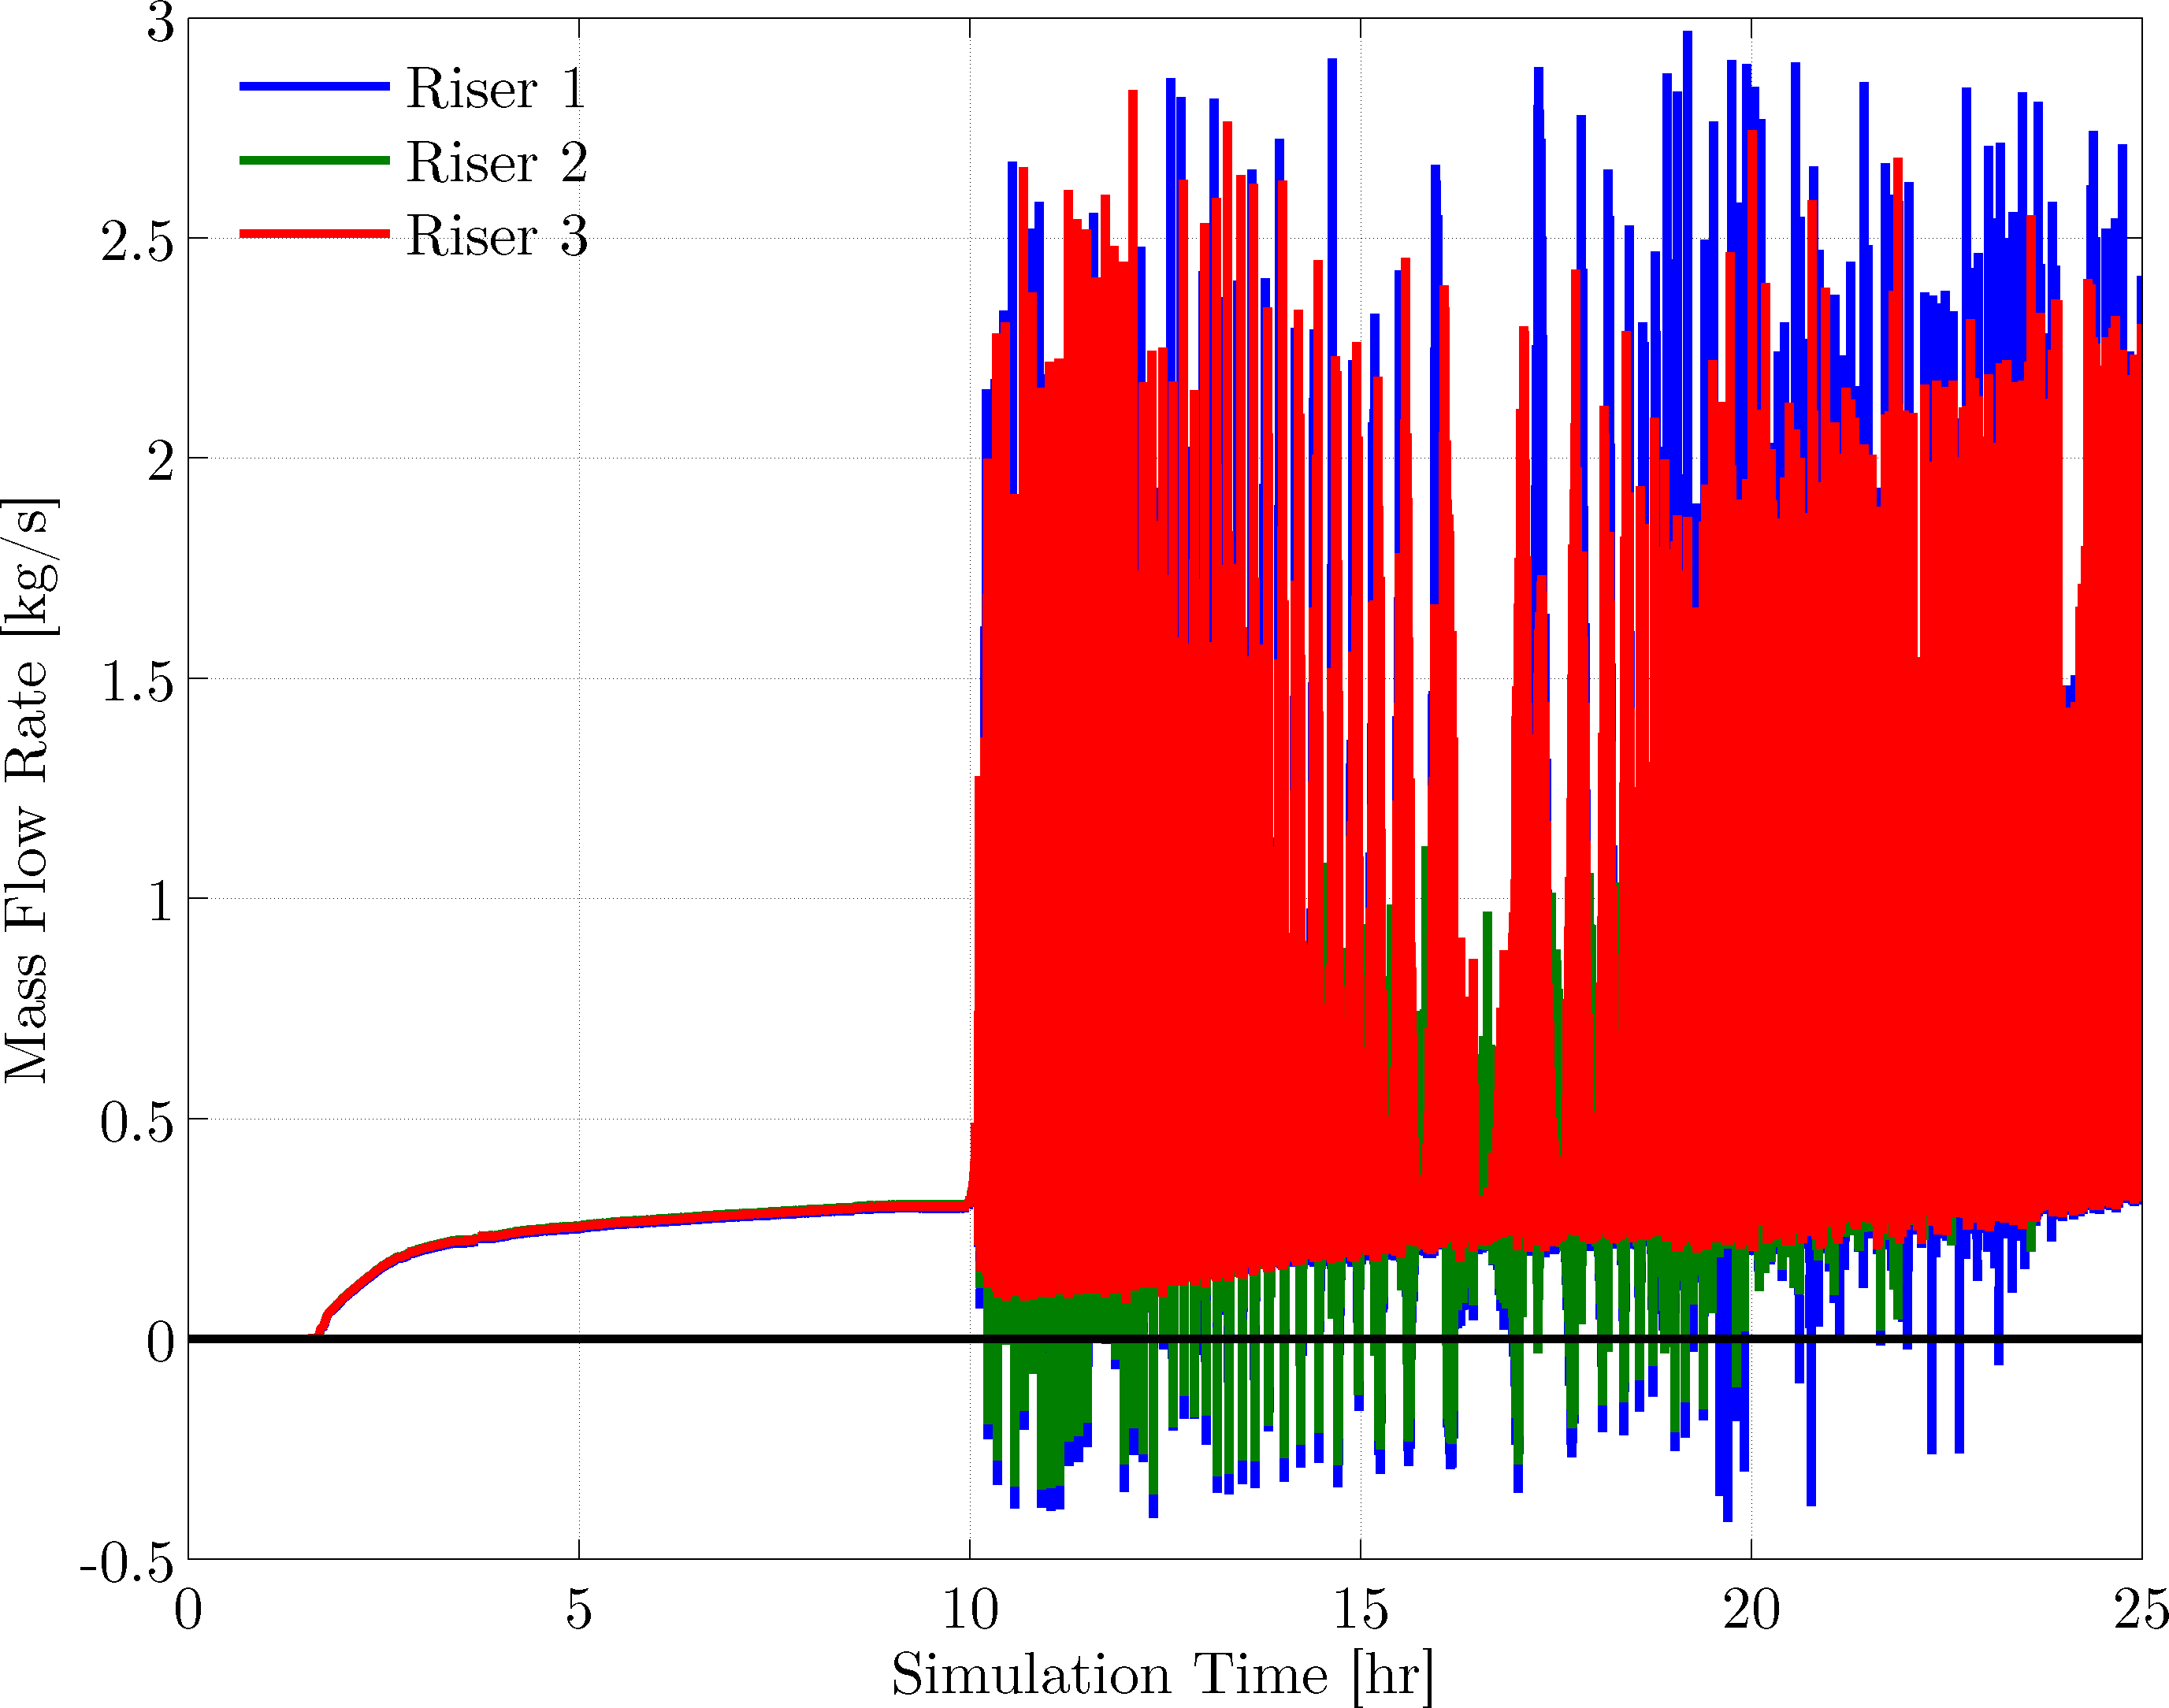
\includegraphics[width=2.7in,angle=0]{ExperimentMassFlowRateVsTime}
            \end{column}
        \end{columns}
    \end{frame}
    
    
% ======================================================= %
%                   Thermohydraulic Theory                %
% ======================================================= %
\subsection{Thermohydraulics}
    \subsubsection*{Conservation Laws}

    % --------------------------------------------------- %
    %                     CLaw: General                   %
    % --------------------------------------------------- %
    \begin{frame}{General Conservation Law (CLaw)}
        Conservation laws balance a vector of conserved variables \qCon over a control volume.\\[2em]
        
        Nonlinear form:
        \begin{equation}
            \pdiff{\qCon}{t} + \pdiff{\FluxFun{\qCon; z,t}}{z}= \SourceFun{\qCon,z,t}
            \label{Eqn:GeneralCLaw}
        \end{equation}
        
        Quasilinear form:
        \begin{equation}
            \pdiff{\qCon}{t} + \pdiff{\FluxFun{\qCon;z,t}}{\qCon}\pdiff{\qCon(z,t)}{z} = \SourceFun{\qCon,z,t}
            \label{Eqn:GeneralCLawQuasilinear}
        \end{equation}
        
        Characteristic speeds:
        \begin{equation}
            \Lambda = \mbox{Eig}\left[\pdiff{\FluxFun{\qCon;z,t}}{\qCon}\right]\label{Eqn:GeneralSpeeds}
        \end{equation}

    \end{frame}
    
    
    % --------------------------------------------------- %
    %                       CLaw: HEM                     %
    % --------------------------------------------------- %
    \subsubsection*{Homogeneous Equilibrium Model}
    \begin{frame}{Homogeneous Equilibrium Model (HEM)}
        Nonlinear form:
        \begin{equation}
            \hspace{-1em}
            \renewcommand*{\arraystretch}{3}
            \pdiff{}{t}\begin{bmatrix}
                            \rho \\
                            \rhou \\
                            \rhoi 
                        \end{bmatrix}
            + 
            \pdiff{}{z}\begin{bmatrix}
                            \rhou                 \\
                            u\,\rhou + P(\rho,i)   \\
                            u\left[\rhoi  + P(\rho,i)\right]
                        \end{bmatrix}
            =  
                        \begin{bmatrix}
                            0 \\% \mdotloss                \\
                            \rho{g(z)} - \frac{\Keff(\qCon)}{2} |\rhou|u  \\
                            \dot{Q}\subs{add}(\qCon,z,t)
                        \end{bmatrix}
            \label{Eqn:HEMStrongConservative}
        \end{equation}
    \end{frame}


    % --------------------------------------------------- %
    %                       CLaw: HEM                     %
    % --------------------------------------------------- %
    \begin{frame}[label=AcousticSpeedsMain]{HEM Speeds}
        Flux Jacobian:
        \begin{equation}
            \renewcommand*{\arraystretch}{2.2}
            \JacobF = 
                \begin{bmatrix}
                    0 & 1 & 0 \\
                    \diff{P}{\rho} - u^2 & 2\,u & \oneo{\rho}\pdiff{P}{i} \\
                    u \left(\diff{P}{\rho} - h\right) & h & u\left(1 + \oneo{\rho}\pdiff{P}{i}\right) 
                \end{bmatrix}
                \label{Eqn:FluxJacobianHEM}
        \end{equation}
        
        Characteristic speeds (\hyperlink{AcousticSpeeds}{plot}):
        %\hypertarget{AcousticSpeeds}{AcousticSpeeds}
        \begin{equation}
            \renewcommand*{\arraystretch}{2.2}
            \hspace{-1em}
            \Speeds\subs{\tiny HEM} =   
                \begin{bmatrix}
                    u \\
                    \left(1 + \oneo{2\rho}\pdiff{P}{i}\right)u  \pm \oneo{2 \rho}\;\Sqrt{4 P(\rho,i) \pdiff{P}{i}+\left(u\pdiff{P}{i}\right)^2 + 4 \rho^2 \pdiff{P}{\rho}}
                \end{bmatrix}
                \label{Eqn:SpeedsHEM}
        \end{equation}
    \end{frame}


    \subsubsection*{Thermodynamics}
    \begin{frame}[label=EOS]{Equation of State}
        \begin{Itemize}
            \item{IAPWS-95 non-ideal equation of state for water}
            \item{Magnificently huge curve fit of Helmholtz free energy potential}
            \item{Natural variables are \rho and $T$}
            \item{Back calculate $T$ from \rho and $i$ (\hyperlink{irhoSpace}{plot})}
        \end{Itemize}
    \end{frame}



\subsection{Steady-state Solver}
    % --------------------------------------------------- %
    %                     Numerics: General               %
    % --------------------------------------------------- %
    \begin{frame}{Collocated Nodal Method {\small(steady-state over simple, closed loop)}}
        Simplest to derive; hardest to solve.
        \begin{equation}\renewcommand{\arraystretch}{2.2}
            \pdiff{\FluxFun{\qCon;z}}{z}
                     =  
            \SourceFun{\qCon,z}
            \label{Eqn:HEMBasicSS}
        \end{equation}
        
        \onslide<2->{
        Integrating from $z_{i}$ to $z_{i+1}$:
            \begin{equation}
                \Flux(\qCon;\Space_{i+1}) - \Flux(\qCon;\Space_i) = \Weight_i \Source(\qCon,\Space_{i}) + \Weight_{i+1} \Source(\qCon,\Space_{i+1}) +   \mathcal{O}(|\Space_{i+1}-\Space_i|^2)
                \label{Eqn:IntegrationTrueSolution}
            \end{equation}
        }
        
        \onslide<3->{
        Residual to drive to $0$:
            \begin{equation}
                \mathbf{R}_i(\qCon) = \left[\Flux(\qCon;\Space_{i+1}) - \Flux(\qCon;\Space_i)\right] -
                        \left[\Weight_i \Source(\qCon,\Space_{i}) + \Weight_{i+1} \Source(\qCon,\Space_{i+1})\right]
                \label{Eqn:IntegrationApproxSolution}
            \end{equation}
        }
    \end{frame}
    
    % --------------------------------------------------- %
    %                     Numerics: General               %
    % --------------------------------------------------- %
    \begin{frame}{Collocated Nodal Method {\small(steady-state over simple, closed loop)}}
        Simple form for arbitrary node count:
        \begin{equation}
            \mathbf{R} = \mathbb{C}_F \Flux - \mathbb{C}_S \Source
        \end{equation}
        
        Connectivity matrices:
        \begin{align}
            \mathbb{C}_* &=  \begin{bmatrix}
                        \mathbf{C}_* & \mathbf{ }   & \mathbf{ } \\
                        \mathbf{ }   & \mathbf{C}_* & \mathbf{ } \\
                        \mathbf{ }   & \mathbf{ }   & \mathbf{C}_* 
                     \end{bmatrix}
            \label{Eqn:SysConnMatrices}
        \end{align}
        
        \begin{columns}
            \begin{column}{0.48\textwidth}
                \begin{align}
                        \mathbf{C}_F &=  
                                \begin{bmatrix}
                                    -1     & +1  &        &        &          \\
                                           & -1  & +1     &        &          \\
                                           &     & \ddots & \ddots &          \\
                                           &     &        &  -1    & +1       \\
                                    1      &     &        &        & -1
                                \end{bmatrix}\notag
                \end{align}
            \end{column}
            \begin{column}{0.48\textwidth}
                \begin{align}
                        \mathbf{C}_S &=  
                                \begin{bmatrix}
                                    \Weight_1 & \Weight_2 &          &              &          \\
                                              & \Weight_2 & \Weight_3 &              &          \\
                                              &          & \ddots   & \ddots       &          \\
                                              &          &          & \Weight_{N-1} & \Weight_N \\
                                    \Weight_1 &          &          &              & \Weight_N
                                \end{bmatrix}\notag
                \end{align}
            \end{column}
        \end{columns}
    \end{frame}
    
    
    
    % --------------------------------------------------- %
    %                     Numerics: General               %
    % --------------------------------------------------- %
    \begin{frame}{Collocated Nodal Method {\small(steady-state over simple, closed loop)}}
        Matrices of this form are singular!
        
        Sweeping approach used for steady-state solver:
        \begin{Itemize}
            \item{Tank state is known.}
            \item{Assume a momentum.}
            \item{Sweep through system back to the tank (nonlinear solver over each control volume).}
            \item{Two possibilities}
                \begin{Itemize}
                    \item{Integrated pressure is less than the tank's: reduce momentum}
                    \item{Integrated pressure is greater than the tank's: increase momentum}
                \end{Itemize}
        \end{Itemize}
        Momentum corrections are made through a secant update using the pressure difference as the minimizer.
    \end{frame}
    
    
    \begin{frame}{Test Problem}
            \begin{columns}[T]
            
                \begin{column}[T]{0.85\textwidth}
                    \begin{Itemize}
                        \item{Single phase}
                        \item{Constant friction factor}
                        \item{$10$ kW load}
                        \item{State:}
                            \begin{Itemize}
                                \item{$P = 101325$ Pa}
                                \item{$T = 300$ K}
                            \end{Itemize}
                    \end{Itemize}
                \end{column}
                \hspace{1em}
                \begin{column}[T]{0.24\textwidth}
                    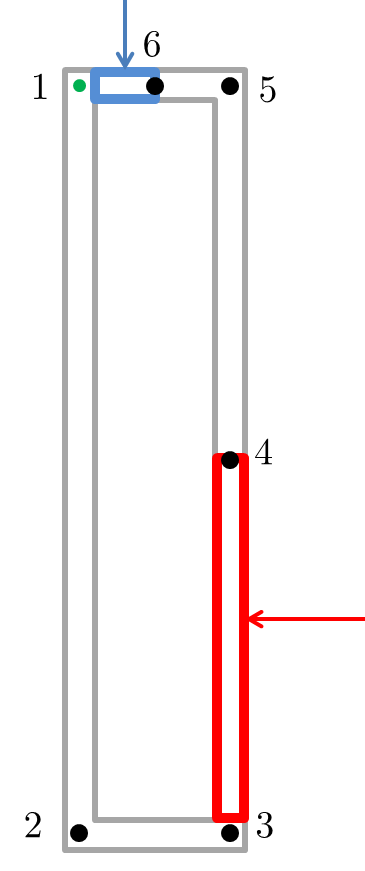
\includegraphics[height=2.4in]{SimpleNatCirc}
                \end{column}
            \end{columns}
        \end{frame}
        
        \begin{frame}{Test Problem}
            \begin{columns}[T]
            
                \begin{column}[T]{0.85\textwidth}
                    \begin{table}[b]%
                        \centering
                        \scriptsize
                        \setstretch{1.4}
                        \rowcolors{2}{}{Gray}
                        \renewcommand{\arraystretch}{1.4}
                        \newcommand{\Solver}{\textbf{Solver}}
                        \newcommand{\Hand}{\textbf{Hand}}
                        \begin{tabular}{ccclcclcc}
                            \toprule
                            \textbf{Measure} & \multicolumn{2}{c}{\textbf{Pressure} [kPa]}       && 
                                               \multicolumn{2}{c}{\textbf{Temperature} [K]}      && 
                                               \multicolumn{2}{c}{\textbf{Density} [kg/m\sups{\tiny 3}]} \\\cmidrule(r){2-9}
                            \textbf{Point}   & \Solver & \Hand  && \Solver & \Hand  && \Solver & \Hand  \\\midrule
                                    1 & 101325 & 101325 && 300.0 & 300   && 996.6 & 996.6\\
                                    2 & 150192 & 150178 && 300.0 & 300   && 996.6 & 996.6\\
                                    3 & 150190 & 150175 && 300.0 & 300   && 996.6 & 996.6\\
                                    4 & 130640 & 130631 && 302.9 & 302.9 && 995.7 & 995.7\\
                                    5 & 101327 & 101328 && 302.9 & 302.9 && 995.7 & 995.7\\
                                    6 & 101326 & 101326 && 302.9 & 302.9 && 995.7 & 995.7\\\bottomrule
                        \end{tabular}
                    \end{table}
                \end{column}
                \hspace{1em}
                \begin{column}[T]{0.24\textwidth}
                    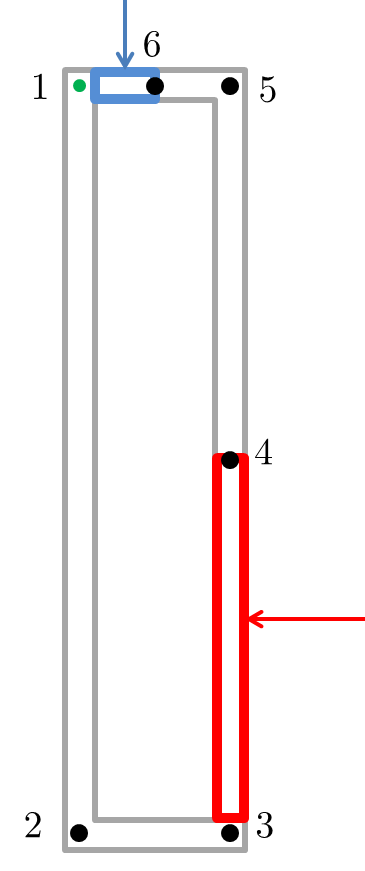
\includegraphics[height=2.4in]{SimpleNatCirc}
                \end{column}
            \end{columns}
            
        \end{frame}
    
    
    
    \subsection{Stability}
    % --------------------------------------------------- %
    %                     Stability: Intro                %
    % --------------------------------------------------- %
    \subsubsection*{Derivation}
    \begin{frame}[label=Perturbation]{Perturbation equations}
        Assumed that the true solution is a summation of a steady-state and a transient
        \begin{equation}
            \qCon(\Space,t) = \qSS(\Space) + \qPer(\Space,t).
        \end{equation}
        
        \onslide<2->{
            General nonlinear perturbation equation (\hyperlink{StabilityDiagrams}{diagrams}):
            \begin{equation}
                \pdiff{\qPer(\Space,t)}{t}  + \pdiff{}{z} \left[\FluxFun{\qSS + \qPer; z,t}\right] = \SourceFun{\qSS + \qPer,z,t} 
                \label{Eqn:NonlinearStabilityEquation}
            \end{equation}
        }
        
        \onslide<3->{
            Taylor expansion about perturbation (neglecting H.O.T.) yields general linear perturbation equation:
            \begin{equation}
                \pdiff{\qPer(\Space,t)}{t}  + \pdiff{}{z}\left[\pdiff{\Flux}{\qSS}\qPer\right] = \pdiff{\Source}{\qSS}\qPer
                \label{Eqn:GeneralLinearizedCLaw}
            \end{equation}
        }
    \end{frame}
    
    % --------------------------------------------------- %
    %                     Stability: Intro                %
    % --------------------------------------------------- %
    \subsubsection*{Linear Solutions}
    \begin{frame}{Solution methods of linear equation}
        Wave form ansatz:
        \begin{equation}
            \widetilde{\qPer} = \qPer^0 \Exp\left[j(\kappa z + \omega t)\right]
            \label{Eqn:WaveForm}
        \end{equation}
        
        \onslide<2->{
        Eigenvalues of dynamical system (piecewise integration around loop):
        \begin{equation}
            \pdiff{\overline{\qPer}}{t} = \mathbb{A}(\qSS,t)\overline{\qPer}
            \label{Eqn:EigenvalueStability}
        \end{equation}
        }
        
        \onslide<3->{
        Laplace transform (zeros of transfer function):
        \begin{equation}
            s \breve{\qPer} - \qPer(z,0) + \pdiff{}{z}\left[\pdiff{\Flux}{\qSS}\breve{\qPer} \right] = \pdiff{\Source}{\qSS}\breve{\qPer} 
            \label{Eqn:LaplaceTransform}
        \end{equation}
        }
    \end{frame}
    
    
    
    \subsubsection*{Test Problem Stability}
    \begin{frame}{Is the Test Problem Stable?}
            \begin{columns}[T]
                \begin{column}[T]{0.85\textwidth}
                    Eigenvalue approach\\[0.50em]
                    Loop Integrated:
                    \begin{equation}
                       \Re(\lambda) =   \begin{bmatrix} 
                                            -0.0531     \\
                                            0 \\
                                            0
                                        \end{bmatrix}
                    \end{equation}\\[0.50em]
                    4-partition Piecewise Integration:
                    \begin{equation}
                        \Re(\lambda) =   \begin{bmatrix} 
                                            \pm 1510        \\
                                            \pm(\pm 346)    \\
                                            \pm 56.2        \\
                                            -0.1            \\
                                            0               \\
                                            0               \\
                                            0
                                        \end{bmatrix}
                    \end{equation}
                \end{column}
                \hspace{1em}
                \begin{column}[T]{0.24\textwidth}
                    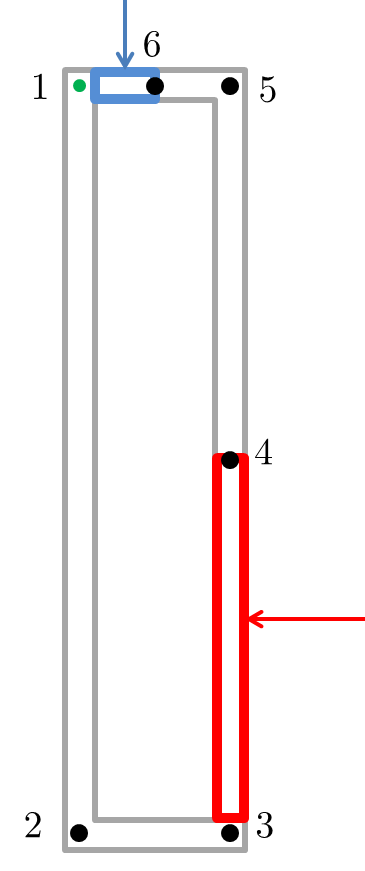
\includegraphics[height=2.4in]{SimpleNatCirc}
                \end{column}
            \end{columns}
    \end{frame}
    
    
\section{Proposed Work}

    % --------------------------------------------------- %
    %                     Numerics: FVM                   %
    % --------------------------------------------------- %
    \subsection*{Current Work}
    \begin{frame}[label=NonrigorMain]{Current Work}
        ``Staggered'': mass and energy equations are integrated over a different space than the momentum equations
        \begin{Itemize}
            \item{Avoids velocity-pressure decoupling}
            \item{Flexible interpretation of momentums: information propagators}
            \item{Allows \hyperlink{Nonrigor}{Non-rigorous grids}}
        \end{Itemize}
        
        \vspace{2em}
        Time integration: Implicit Euler
        \begin{Itemize}
            \item{Unconditionally stable and TVD}
            \item{Very diffusive}
        \end{Itemize}
    \end{frame}

    \begin{frame}{Semidiscrete, Donor-Cell equations}
        \begin{subequations}\label{Eqn:Semidiscrete1}
            Momentum cells have a ``from'' and ``to'' for handedness.
            Donor quantities depend on sign of momentum.
            
            \begin{align}
                \pdiff{\rho\subs{k}}{t}  &= - \oneo{\CVvol}\sum{\rhou\subs{d} A\subs{d}}\\[1em]
                \pdiff{\rhoi\subs{k}}{t} &= - \oneo{\CVvol}\sum{u_d\left[\rhoi_d  + P(\rho_d,i_d)\right] A\subs{k}} + \dot{Q}\subs{add,k}(\qCon,z,t) \\[1em]
                \pdiff{\rhou\subs{m}}{t} &= - \oneo{\MCvol}\left[u\,\rhou\rvert^\text{to}_\text{from} + P_\text{to} - P_\text{from}\right]A\subs{m} + \\
                                         &  \qquad\qquad  \frac{A\subs{m}}{\MCvol}
                                               \int_{\text{from}}^{\text{to}}\left[\rho{g(z)} - \frac{\Keff(\qCon)}{2} u\,|\rhou|\right] \mathrm{d}s \notag
            \end{align}
        \end{subequations}
    \end{frame}


    \subsection*{Goals}
    \begin{frame}{Goals}
        Path Forward:
            \begin{Itemize}
                \item{Complete transient, HEM solver}
                \item{Look at HEM boiling behavior}
                \item{Attain true non-simple, closed-loop steady-state calculations}
            \end{Itemize}
            \vfill
        Outcomes
            \begin{Itemize}
                \item{Look at }
                \item{Examine the quasi-steady stability of the RCCS experiment}
                \item{Stability maps of the three-riser system, in general, for various parameters}
                \item{Analytical and physical understanding of how boil-off affects flow behavior}
            \end{Itemize}
    \end{frame}
    
    \subsection*{Goals with Pictures}
    \begin{frame}[c]{Path Goals ... with Pictures!}
        \begin{columns}[c]
            \hspace{1em}
            \begin{column}[c]{0.6\textwidth}
                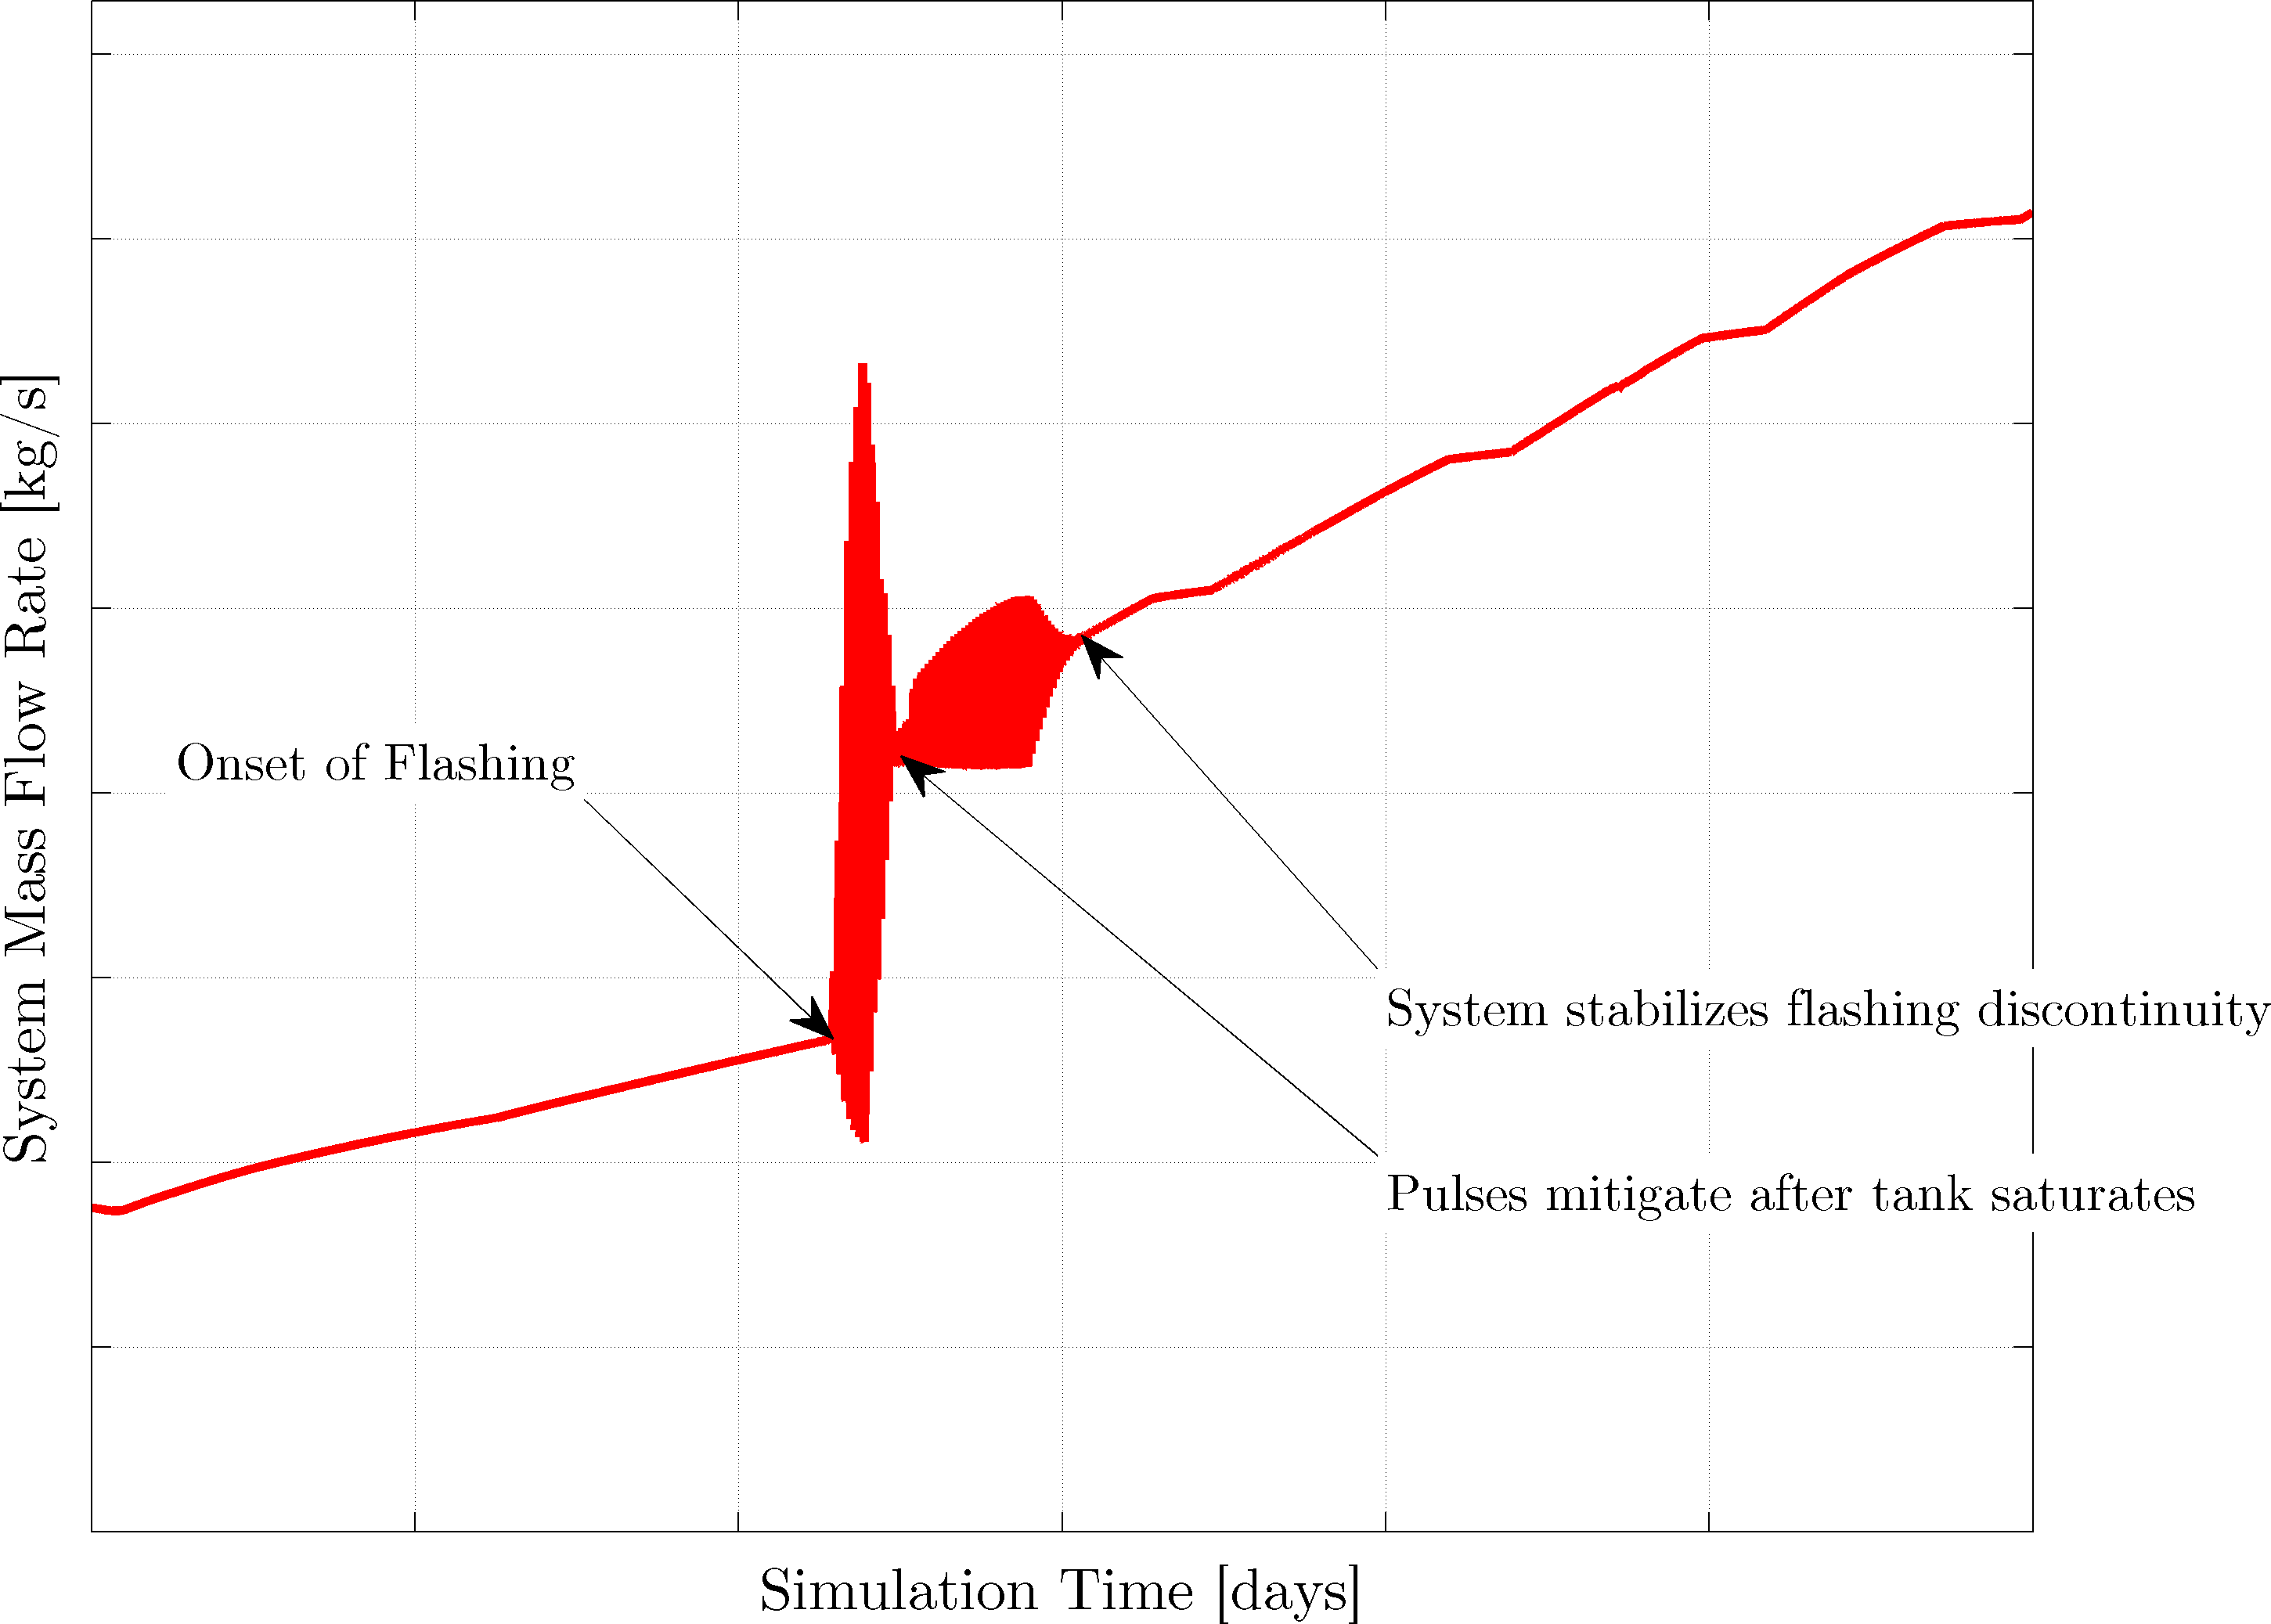
\includegraphics[height=1.60in]{PowerProfiles_MassFlowRateAnnotationsThesis}
            \end{column}
            \begin{column}[c]{0.6\textwidth}
                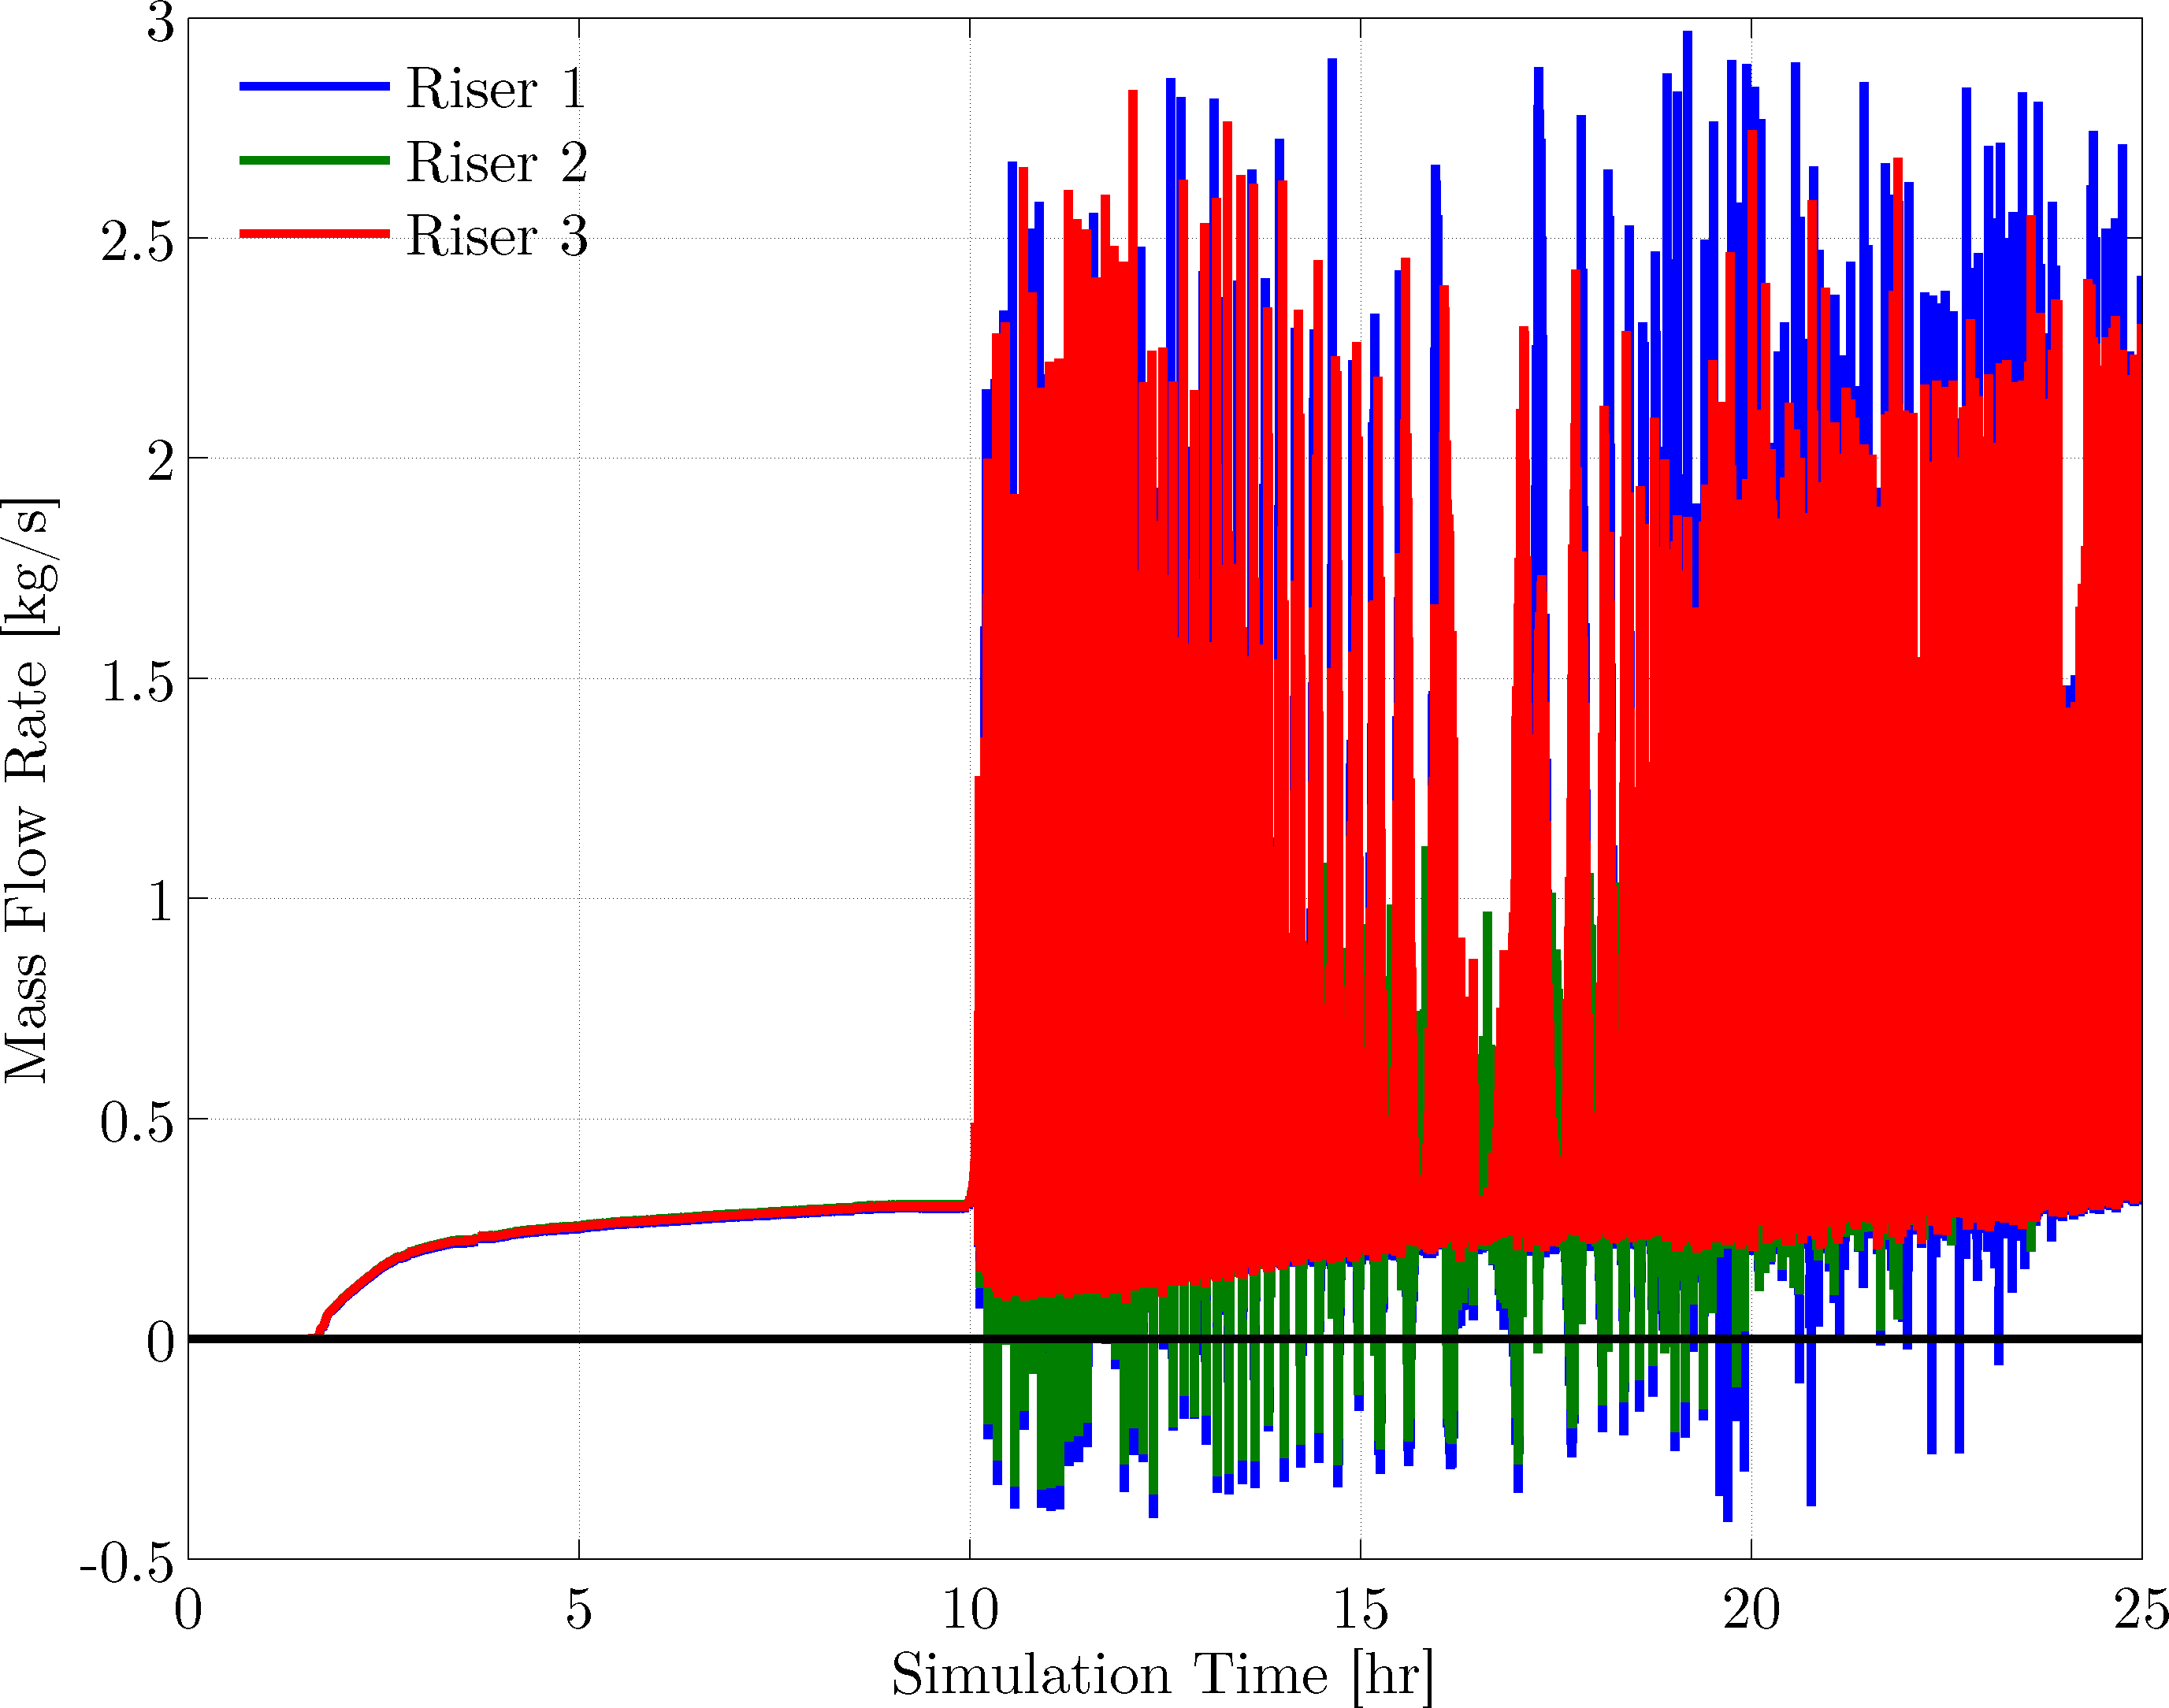
\includegraphics[height=1.60in]{ExperimentMassFlowRateVsTime}
            \end{column}
        \end{columns}
    \end{frame}
    
    
    \subsection*{Acknowledgements}
    \begin{frame}[c]{Acknowledgements}
        \begin{center}
                NEUP Program and NRC Fellowship.
        \end{center}
    \end{frame}
        

    \subsection*{End}
    \begin{frame}[c]{Questions}
        \begin{center}
                ``The key to wisdom is this: constant and frequent questioning. 
                  For by doubting we are led to question, and by questioning we arrive at the truth.''\\
                \hfill --- Peter Abelard
        \end{center}
    \end{frame}



% ======================================================= %
%                       Appendix                          %
% ======================================================= %
\appendix
    
    
    \section{Supplements}
    
    
    % ====================================================================== %
    %                           Stagger/Collocated                           %
    % ====================================================================== %
    \subsection*{Staggered/Collocated}
    \begin{frame}[c,label=Meshes]{Staggered/Collocated}
        \begin{columns}
            \begin{column}[T]{0.4\textwidth}
                Staggered mesh:                
               \begin{center}
                   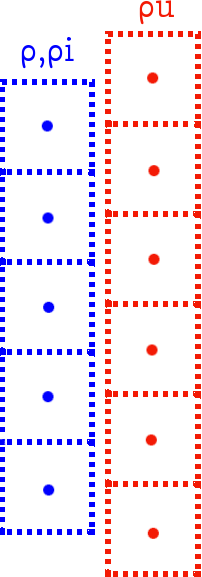
\includegraphics[height=2.2in]{StaggeredMesh}
               \end{center}
            \end{column}
            \hfill
            \begin{column}[T]{0.4\textwidth}
                Collocated mesh:
                \begin{center}
                    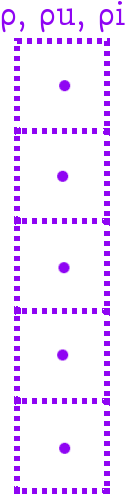
\includegraphics[height=2.2in]{CollocatedMesh}
                \end{center}
            \end{column}
        \end{columns}
    \end{frame}
    
    
    % ====================================================================== %
    %                      Rigorous/Non-rigorous                             %
    % ====================================================================== %
    \subsection*{Rigorous vs. Nonrigorous}
    \begin{frame}[c,label=Nonrigor]{Rigorous vs. Non-Rigorous}\label{Rigorous}
        \begin{columns}
            \begin{column}[T]{0.4\textwidth}
                Rigorous staggered mesh (CFD):                
               \begin{center}
                   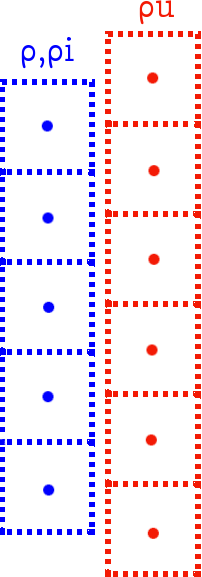
\includegraphics[height=2.2in]{StaggeredMesh}
               \end{center}
            \end{column}
            \hfill
            \begin{column}[T]{0.4\textwidth}
                Non-rigorous staggered mesh (System codes):
                \begin{center}
                    \null\vfill
                    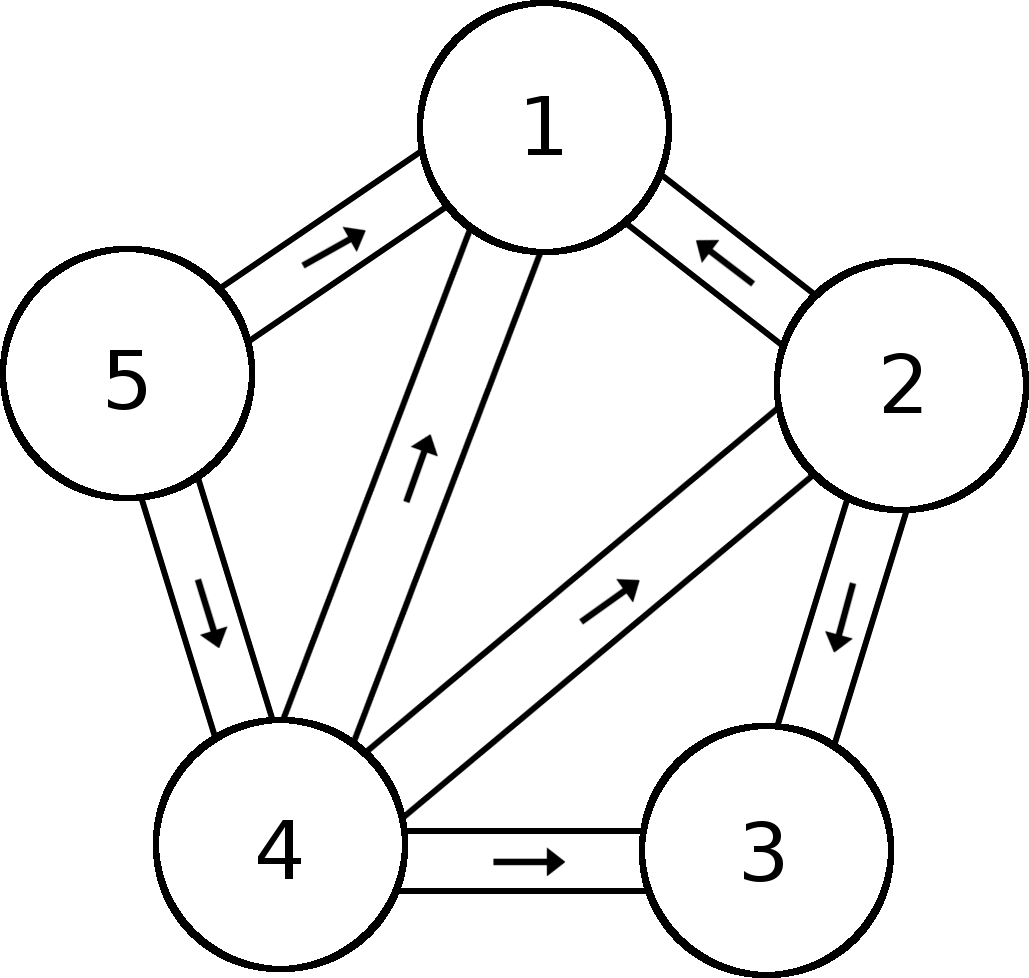
\includegraphics[scale=0.325]{NonrigorousMesh}
                    \null\vfill
                \end{center}
                \hfill\textit{\tiny\hyperlink{NonrigorMain}{return}}
            \end{column}
        \end{columns}
    \end{frame}
    
    
    % ====================================================================== %
    %                          Acoustic Speeds                               %
    % ====================================================================== %
    \subsection*{Acoustic Speeds}
    \begin{frame}[c,label=AcousticSpeeds]{Acoustic Speeds}
       \begin{center}
            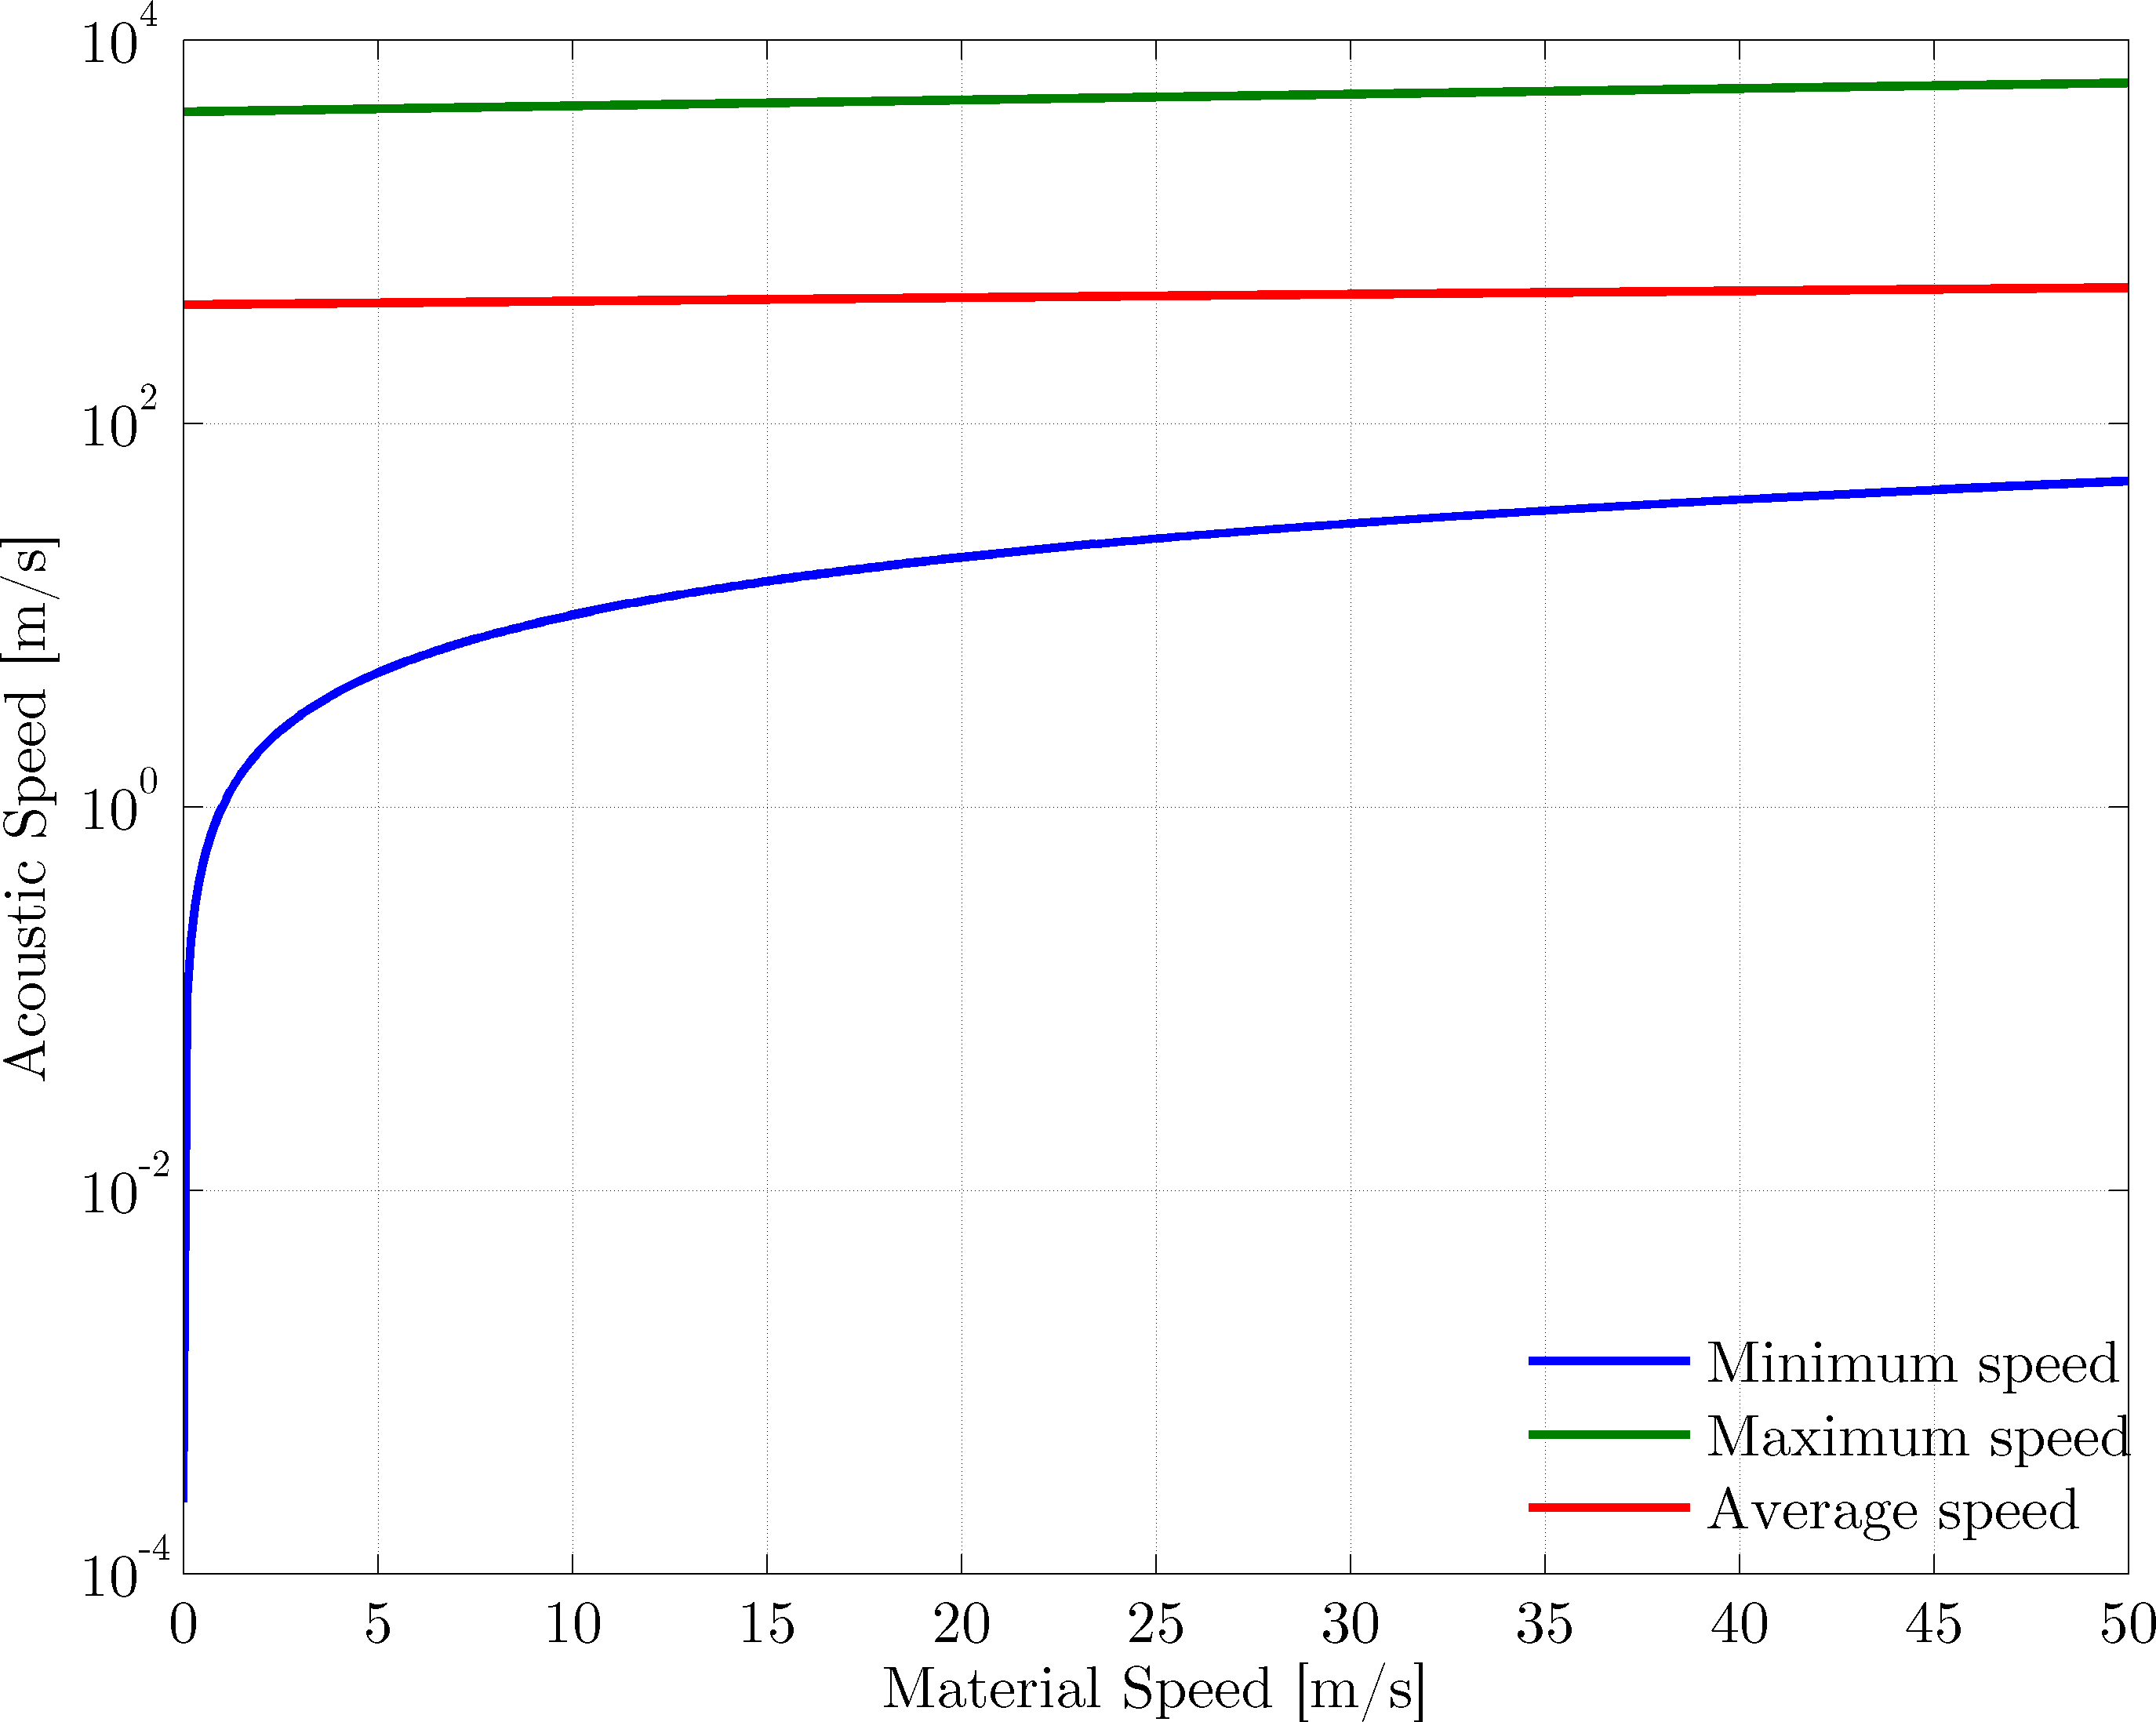
\includegraphics[height=2.2in]{AcousticSpeedVsMaterialSpeed}
       \end{center}
        \hfill\textit{\tiny\hyperlink{AcousticSpeedsMain}{return}}
    \end{frame}



    % ====================================================================== %
    %                          Non-simple, closed loop                       %
    % ====================================================================== %
    \subsection*{Non-simple, closed loop}
    \begin{frame}[c,label=NonsimpleClosedLoop]{Non-simple, closed loop}
        \begin{center}
            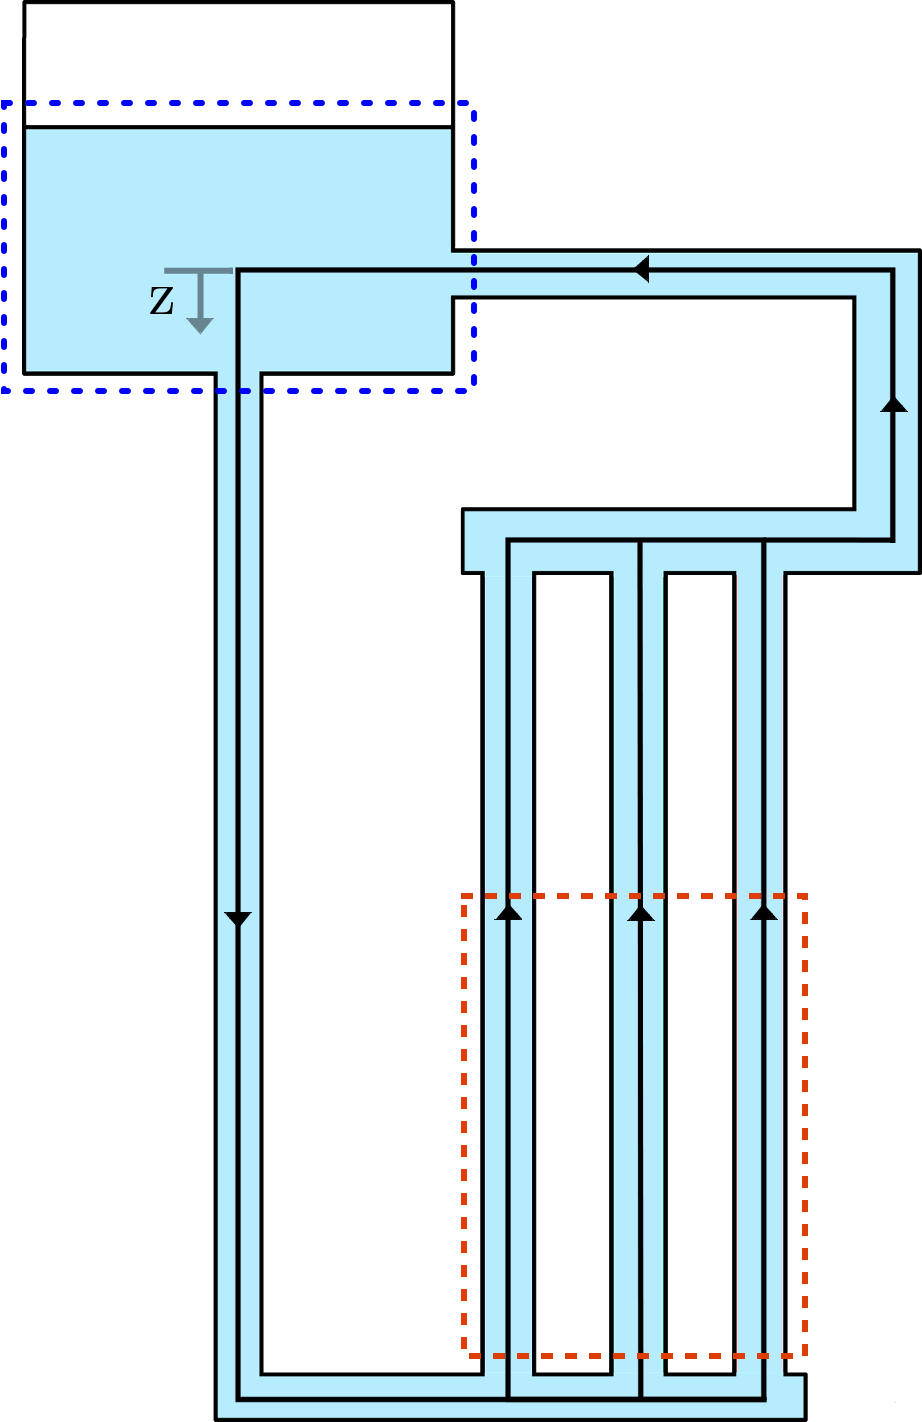
\includegraphics[height=2.2in]{ComputationalGeometry}
        \end{center}
    \end{frame}
    
    
    % ====================================================================== %
    %                          Non-simple, closed loop                       %
    % ====================================================================== %
    \subsection*{i-rho Space}
    \begin{frame}[c,label=irhoSpace]{$i$-\rho Diagram}
        \begin{center}
            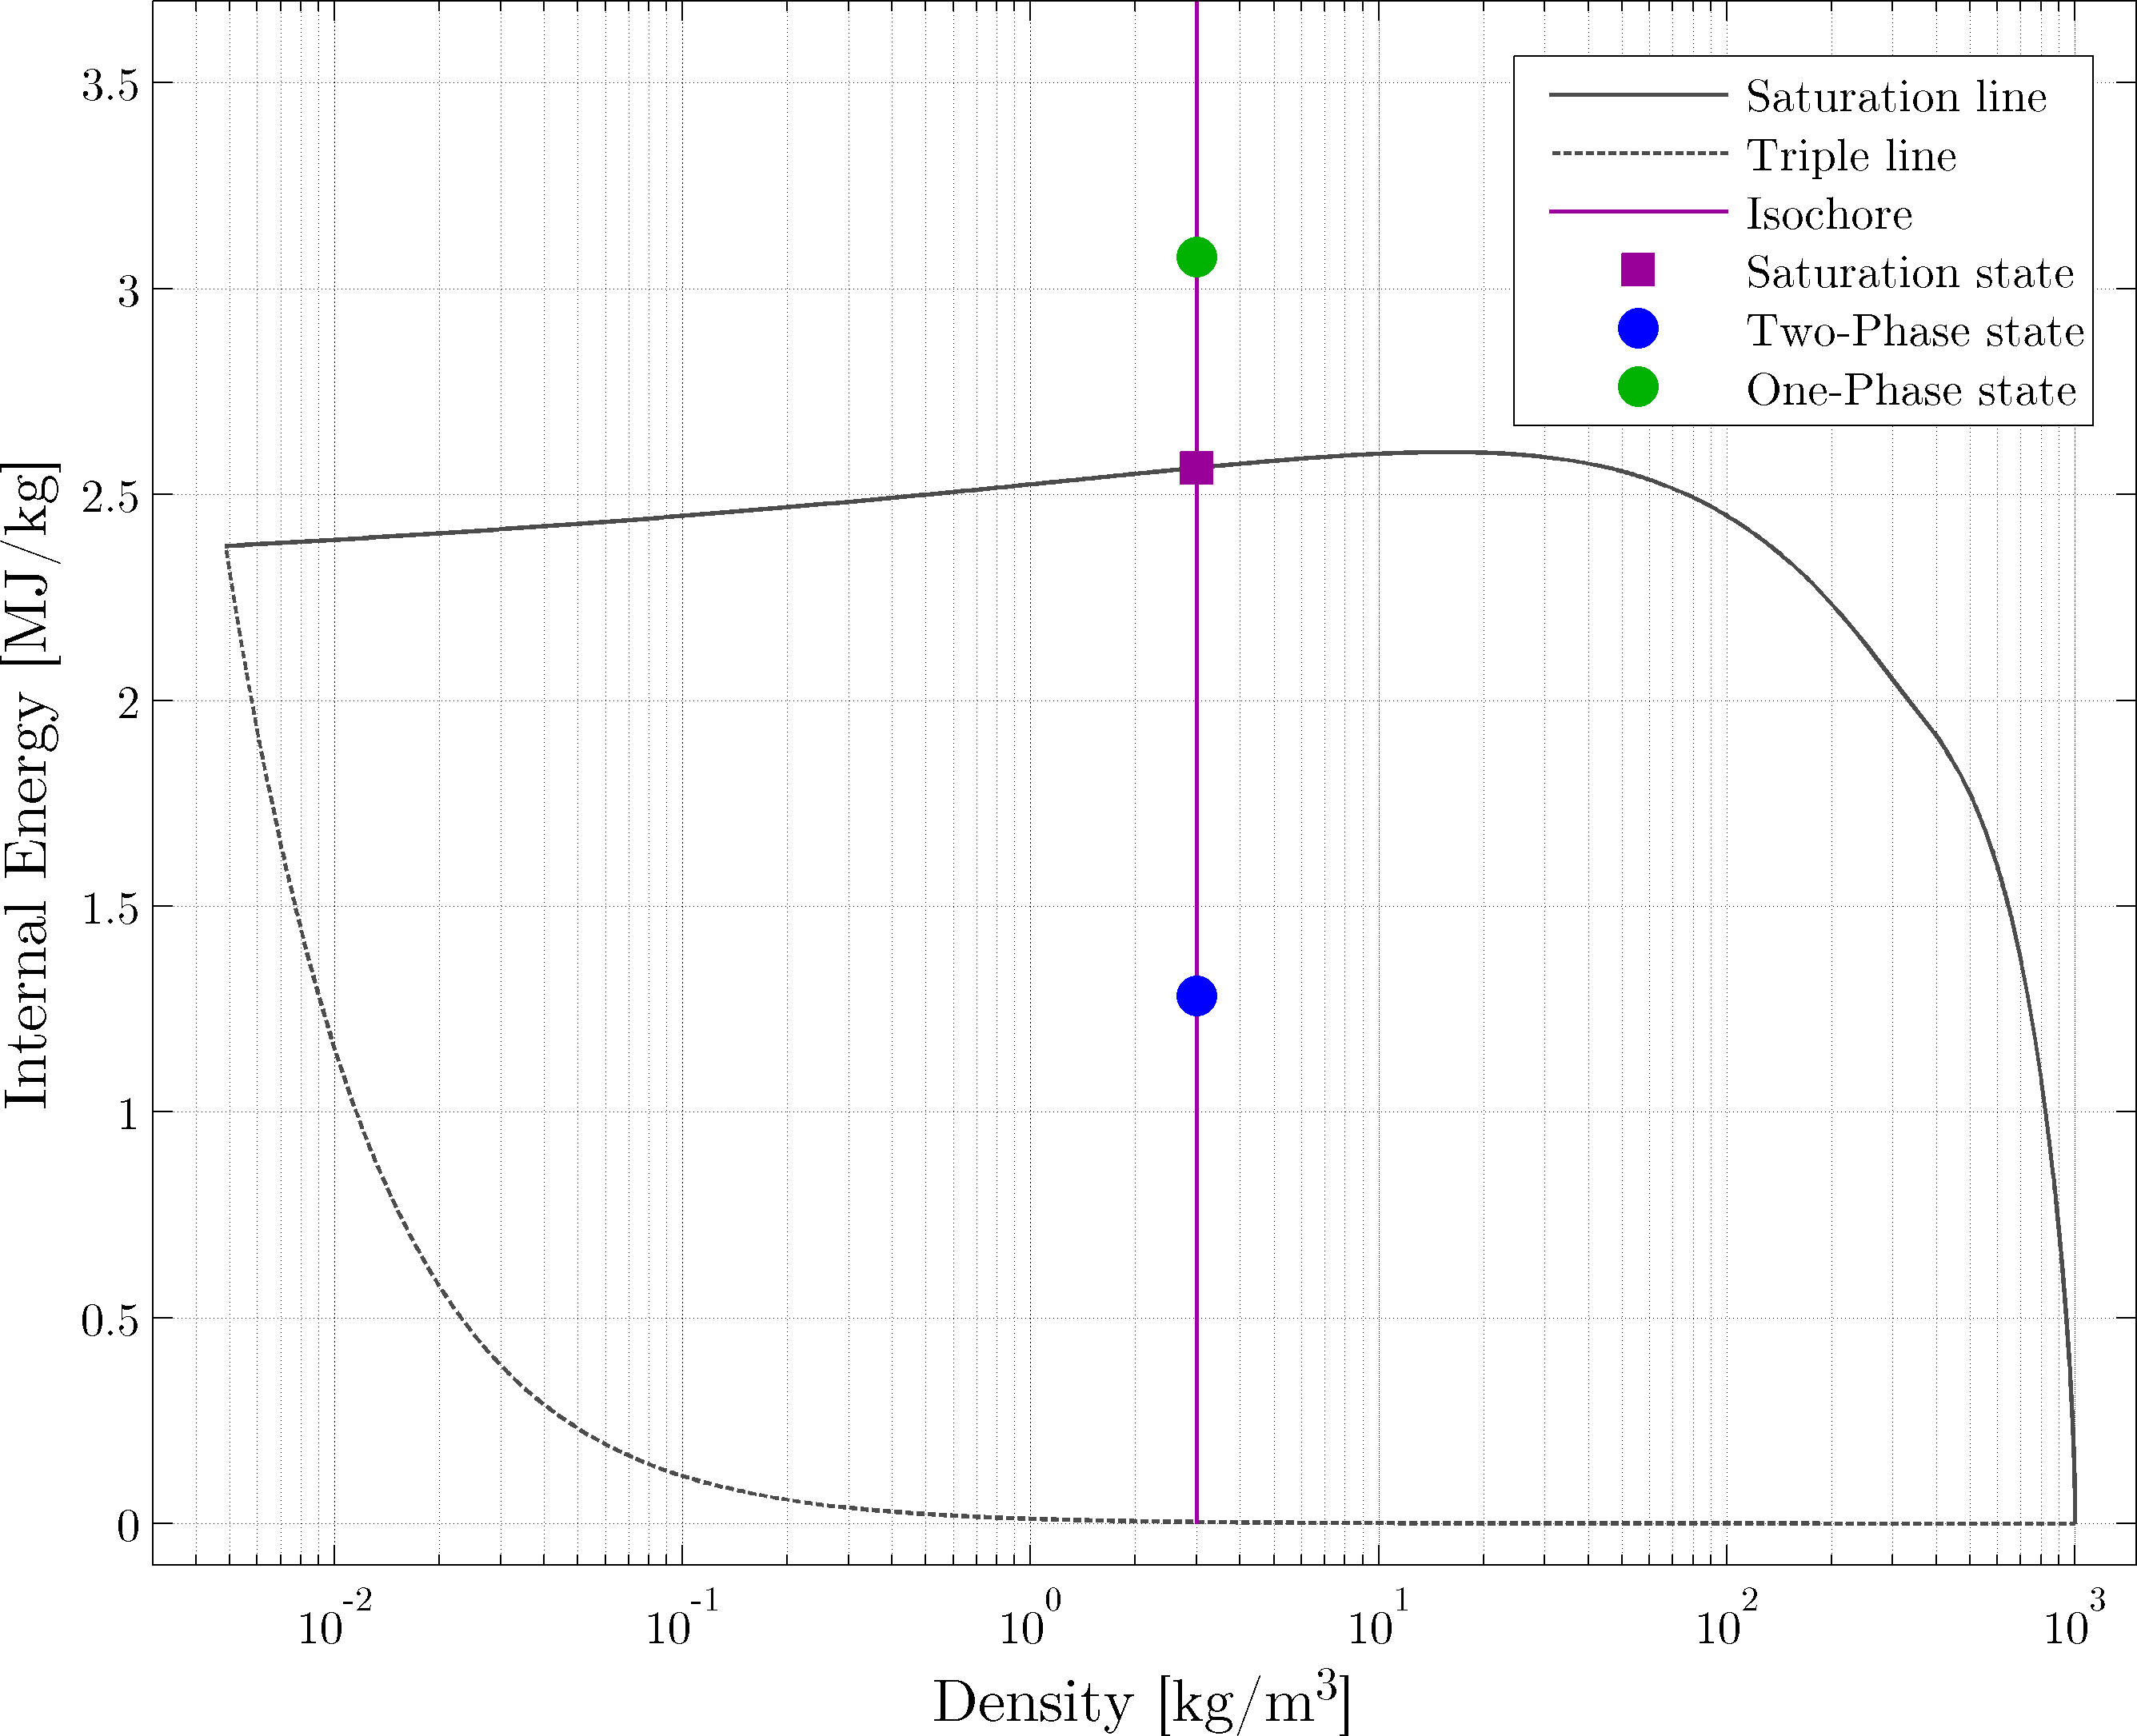
\includegraphics[height=2.2in]{InteEnergyVsDensity}
        \end{center}
        \hfill\textit{\tiny\hyperlink{EOS}{return}}
    \end{frame}
    
    
    
    % ====================================================================== %
    %                            Stability Diagrams                          %
    % ====================================================================== %
    \subsection*{Stability Diagrams}
    \begin{frame}[c,label=StabilityDiagrams]{Stability Diagrams}
        \begin{columns}
            \begin{column}[T]{0.4\textwidth}
                Linearly stable, nonlinearly unstable:
                \begin{center}
                    \vspace{0.09in}
                    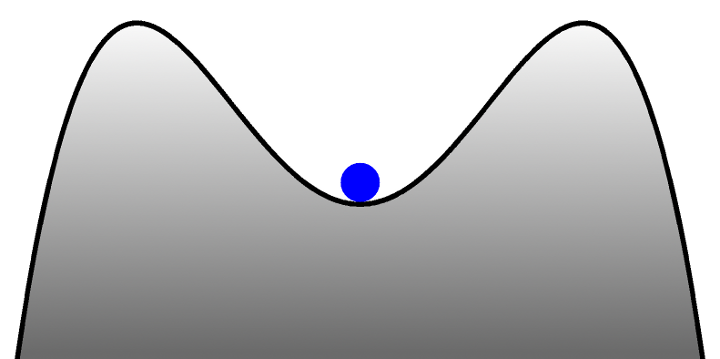
\includegraphics[height=0.91in]{LinearlyStableNonlinearlyUnstable}
                \end{center}
            \end{column}
            \hfill
            \begin{column}[T]{0.4\textwidth}
                Linearly unstable, nonlinearly stable:
                \begin{center}
                    \null\vfill
                    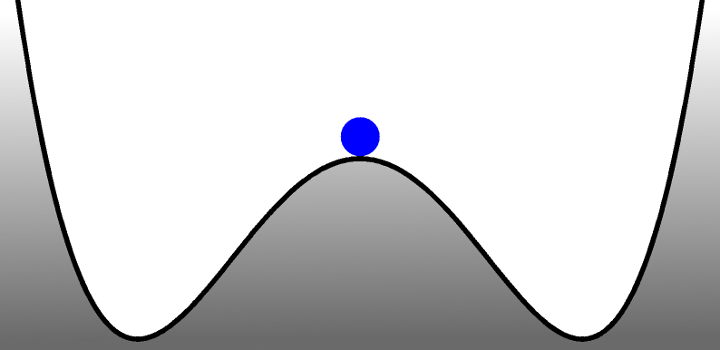
\includegraphics[height=0.83in]{LinearlyUnstableNonlinearlyStable}
                    \null\vfill
                \end{center}
                \hfill\textit{\tiny\hyperlink{Perturbation}{return}}
            \end{column}
        \end{columns}
    \end{frame} 
    
    
    
    % ====================================================================== %
    %                            Stability Diagrams                          %
    % ====================================================================== %
    \subsection*{System Mass flow: 4 days}
    \begin{frame}[c,label=MassFlow4Days]{System Mass flow: 4 days}
        \begin{center}
            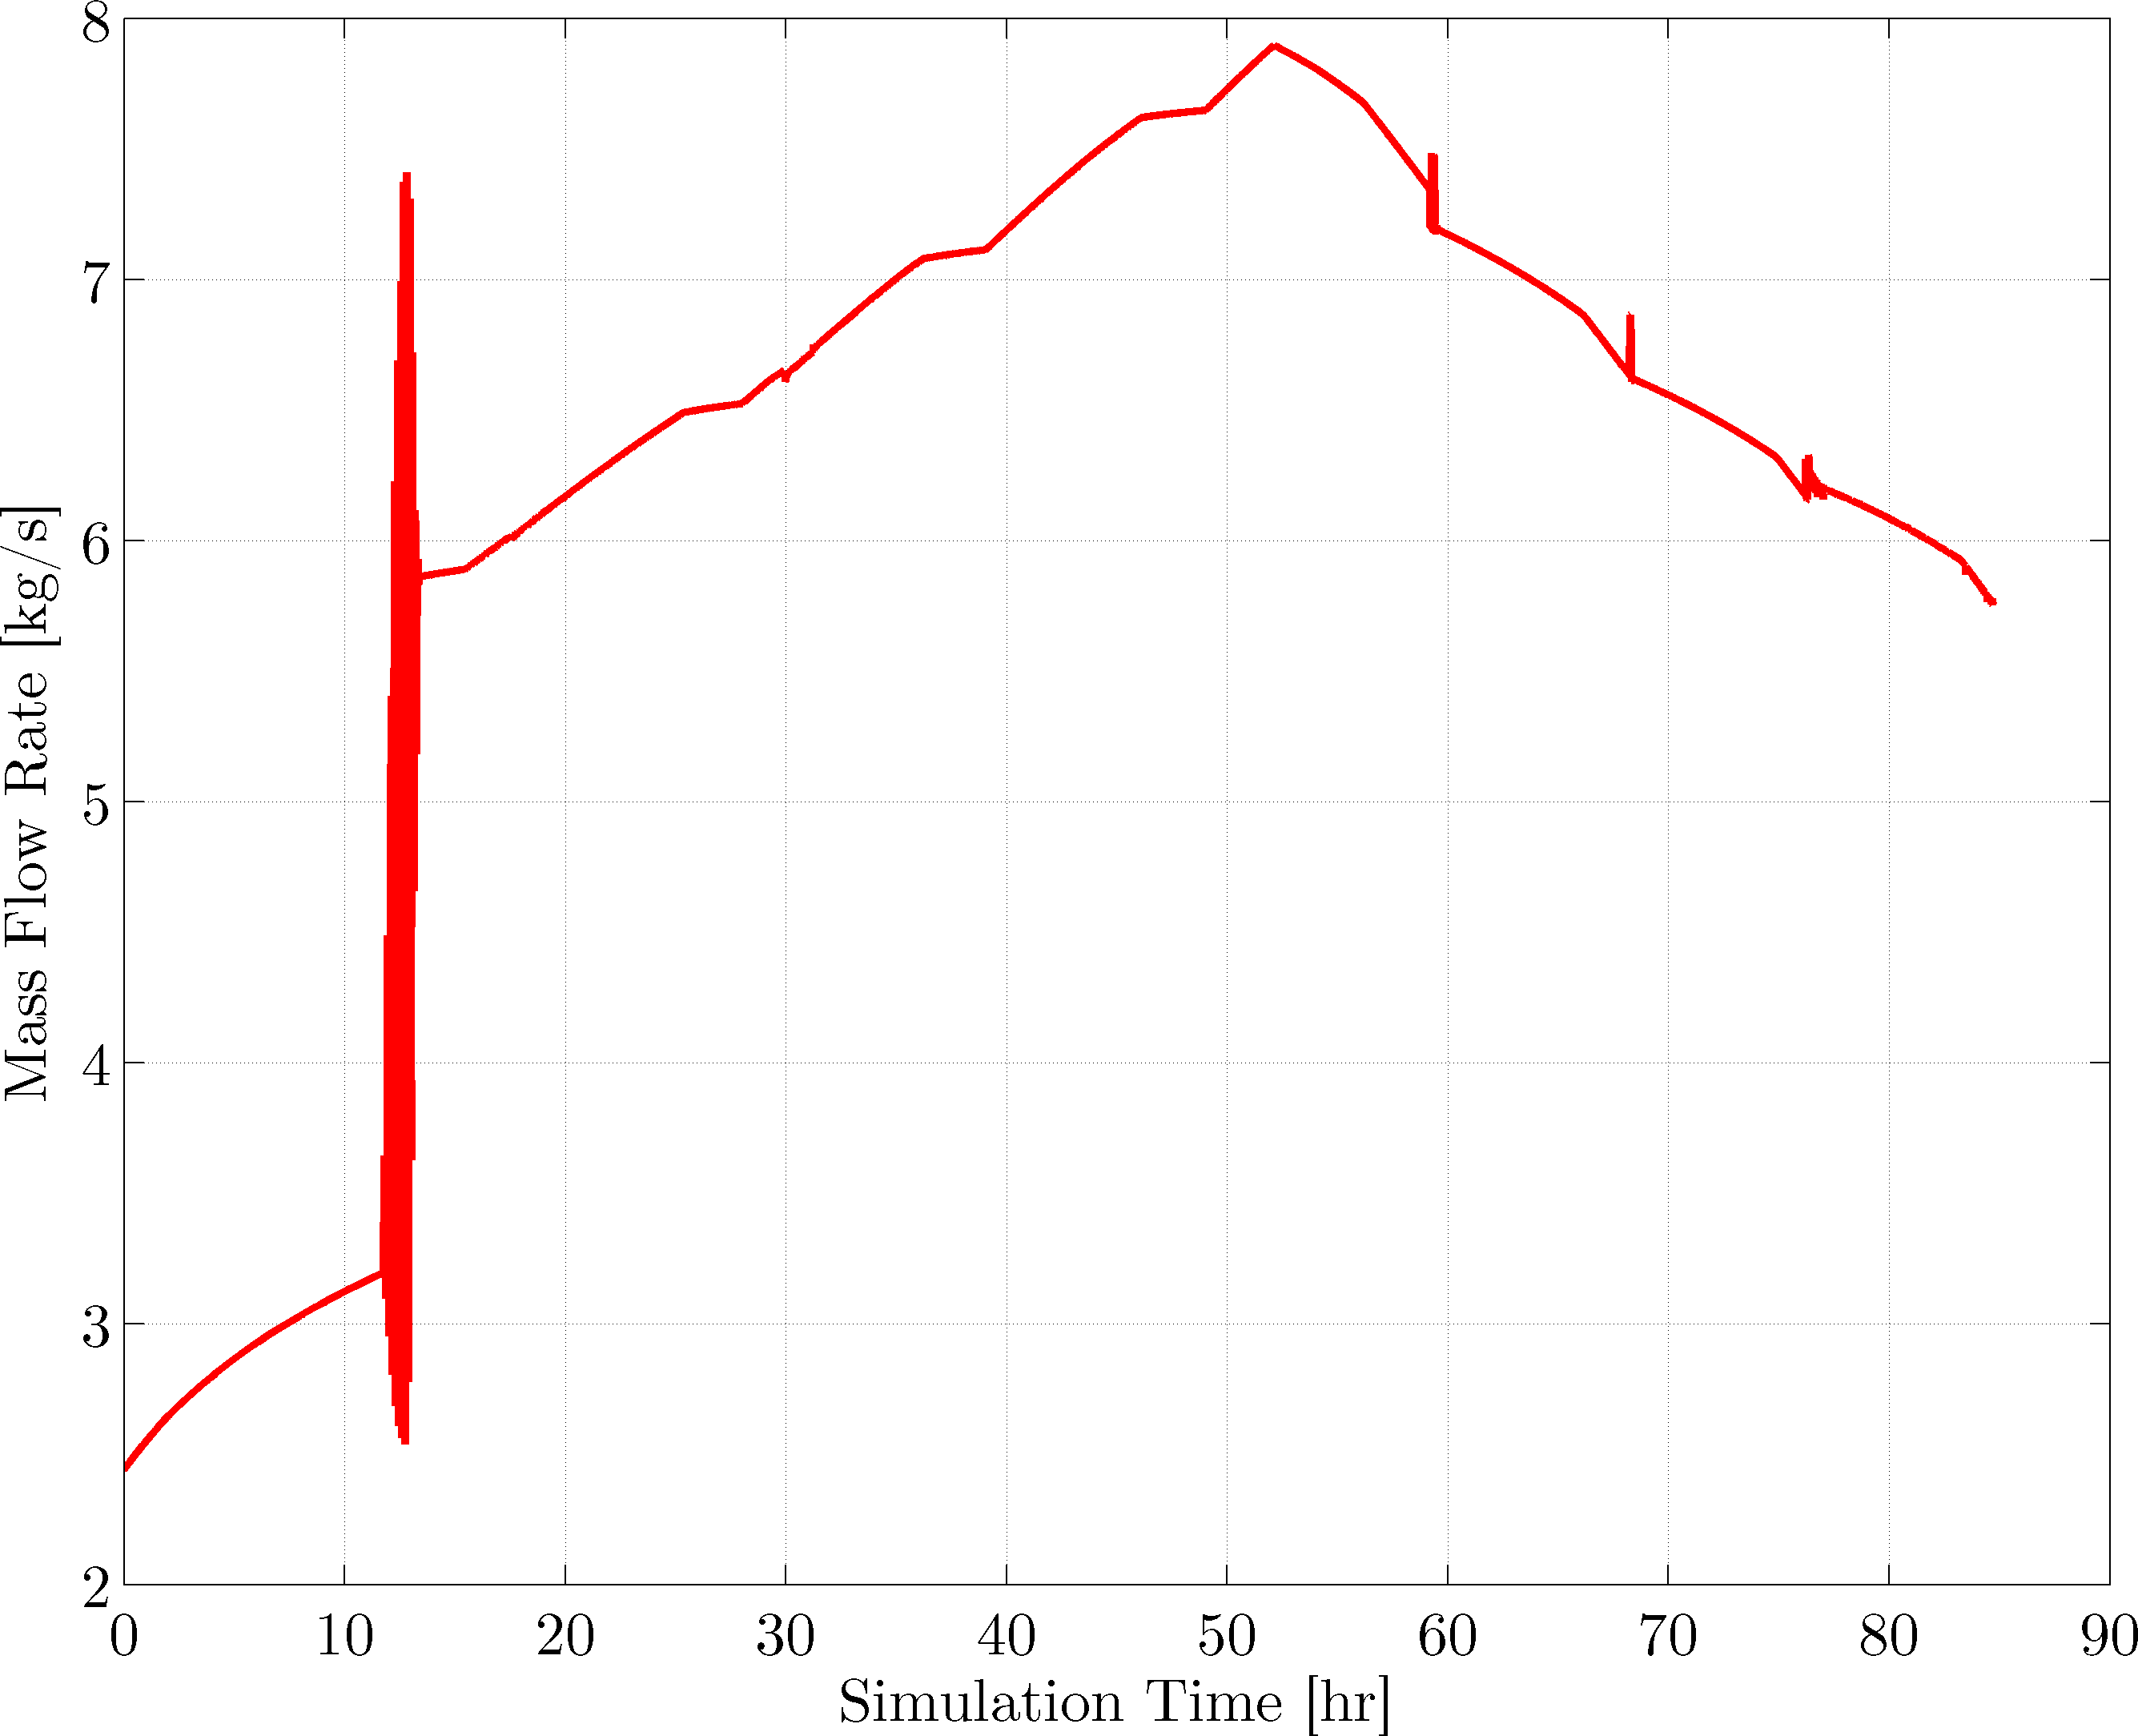
\includegraphics[height=2.4in]{MassRateFor4days}
        \end{center}
        \hfill\textit{\tiny\hyperlink{MassFlowAnnotate}{return}}
    \end{frame}
    
    
    
    % ====================================================================== %
    %                             Multiphase Model                           %
    % ====================================================================== %
    \subsection*{Multiphase Model}
    \begin{frame}[label=Multiphase]{Multiphase Model}
         \begin{equation}
            \renewcommand{\arraystretch}{2.2}
            \pdiff{}{t}\begin{bmatrix}
                           \rhok \\
                           \rhouk \\
                           \rhoik 
                        \end{bmatrix}
            + 
            \pdiff{}{z}\begin{bmatrix}
                            \rhouk                 \\
                            \uk\,    \rhouk  + P(\rho\subs{\phi},\ik)   \\
                            \uk\left[\rhoik  + P(\rho\subs{\phi},\ik)\right]
                        \end{bmatrix}
                     = 
        \end{equation}
        \begin{equation}\renewcommand{\arraystretch}{2.2}
            \begin{bmatrix}
                \mathbb{M}\subs{\phi} \\
                \rhok{g(z)} - \frac{\Keff\subs{,\phi}(\qCon)}{2} \uk\,|\rhouk| + \mathbb{P}\subs{\phi}  \\
                \dot{Q}\subs{add,\phi}(\qCon,z,t) + \mathbb{E}\subs{\phi}
            \end{bmatrix}
            \notag
        \end{equation}
    \end{frame}


\end{document}

